\documentclass[10pt,a4paper]{article}
\usepackage[utf8]{inputenc}
\usepackage{amsmath}
\usepackage{amsfonts}
\usepackage{amssymb}
\usepackage{amsthm}
\usepackage{float}
\usepackage{mathtools}
\usepackage{geometry}[margin=1in]
\usepackage{xspace}
\usepackage{tikz}
\usepackage{mathrsfs}
\usetikzlibrary{shapes, arrows, decorations.pathmorphing}
\usepackage[parfill]{parskip}
\usepackage{subcaption}
\usepackage{stmaryrd}
\usepackage{marvosym}
\usepackage{dsfont}

\newcommand{\st}{\text{ s.t. }}
\newcommand{\contr}{\lightning}
\newcommand{\im}{\mathfrak{i}}
\newcommand{\R}{\mathbb{R}}
\newcommand{\Q}{\mathbb{Q}}
\newcommand{\C}{\mathbb{C}}
\newcommand{\F}{\mathbb{F}}
\newcommand{\K}{\mathbb{K}}
\newcommand{\N}{\mathbb{N}}
\newcommand{\Z}{\mathbb{Z}}
\renewcommand{\H}{\mathds{H}}
\newcommand{\nequiv}{\not\equiv}
\newcommand{\powset}{\mathcal{P}}
\renewcommand{\th}[1][th]{\textsuperscript{#1}\xspace}
\newcommand{\from}{\leftarrow}
\newcommand{\legendre}[2]{\left(\frac{#1}{#2}\right)}
\newcommand{\ow}{\text{otherwise}}
\newcommand{\imp}[2]{\underline{\textit{#1.}$\implies$\textit{#2.}}}
\let\oldexists\exists
\renewcommand{\exists}{\oldexists\;}
\renewcommand{\hat}{\widehat}
\renewcommand{\tilde}{\widetilde}
\newcommand{\one}{\mathds{1}}
\newcommand{\under}{\backslash}
\newcommand{\injection}{\hookrightarrow}
\newcommand{\surjection}{\twoheadrightarrow}
\newcommand{\jacobi}{\legendre}
\newcommand{\floor}[1]{\lfloor #1 \rfloor}
\newcommand{\ceil}[1]{\lceil #1 \rceil}
\newcommand{\cbrt}[1]{\sqrt[3]{#1}}

\DeclareMathOperator{\ex}{ex}
\DeclareMathOperator{\id}{id}
\DeclareMathOperator{\upper}{Upper}
\DeclareMathOperator{\dom}{dom}

\DeclareMathOperator{\charr}{char}
\DeclareMathOperator{\Image}{im}
\DeclareMathOperator{\ord}{ord}
\DeclareMathOperator{\lcm}{lcm}
\let\emph\relax
\DeclareTextFontCommand{\emph}{\bfseries\em}

\newtheorem{theorem}{Theorem}[section]
\newtheorem{lemma}[theorem]{Lemma}
\newtheorem{corollary}[theorem]{Corollary}
\newtheorem{proposition}[theorem]{Proposition}
\newtheorem{conjecture}[theorem]{Conjecture}

\tikzset{sketch/.style={decorate,
 decoration={random steps, amplitude=1pt, segment length=5pt}, 
 line join=round, draw=black!80, very thick, fill=#1
}}

\title{Coding \& Cryptography}
\begin{document}
\maketitle

\setcounter{section}{-1}
\section{Communication Channels}
This course will be about modelling communication. In general, we have the following idea:

\begin{figure}[H]
\centering

\begin{tikzpicture}
\node (s) at (0,0) {\textsc{Source}};
\node (e) at (4,0) {\textsc{Encoder}};
\node (d) at (8,0) {\textsc{Decoder}};
\node (r) at (12,0) {\textsc{Receiver}};
\draw (s) edge[->] (e) (d) edge[->] (r);
\draw[->, decorate, line join=round, decoration={zigzag, segment length=4, amplitude=0.9, post=lineto, post length=2pt}] (e) -- node[above] {\textsc{Channel}} node[below] {Errors, Noise} (d) ;
\end{tikzpicture}
\end{figure}
\vspace{-1em}
For example, the channel might be an optical or electrical telegraph, modems, audio CDs, satellite relays. The encoding and decoding might be something like \textsc{Ascii}, so that each character in the email ``Call at 2pm" would be encoded into 8 bits using $a = 1100101, \ldots$, giving an 84 bit message to be transmitted via the internet, and decoded by the receiver's email client. Our general aim here will be, given some source and channel (modelled probabilistically), to design an encoder and decoder to send messages economically and reliably.

\underline{Examples}
\begin{itemize}
\item (Noiseless coding) Morse Code. In this code, more common letters are assigned shorter codes, so that we have $A = \cdot - \ast, E = \cdot \ast, Q = - - \cdot - \ast, Z = - - \cdot \cdot \ast$. This is adapted to the \textit{source}, in the sense that we chose the codes based off the expected distribution of letters that we will have to transmit.

\item (Noisy coding) \textsc{Isbn}. In the \textsc{Isbn} encoding, every book is given a 10 digit number $a_1a_2\ldots a_{10}$, with $\sum_{i=1}^{10} (11-i)a_i \equiv 0 \mod 11$. This is adapted to the \textit{channel}, in the sense that the likely errors to occur will be 1 incorrect digit, or accidentally transposing two digits, which this code is resistant to (will return an error rather than an erroneous result).
\end{itemize}

A \emph{communication channel} accepts symbols from some alphabet $\mathscr{A} = \{a_1, a_2, \ldots, a_r\}$ (e.g. $\{0,1\}, \{a,b,\ldots,z\}$), and outputs symbols from an alphabet $\mathscr{B} = \{b_1, \ldots, b_s\}$. The channel is modelled by the probabilities:
\begin{center}$\P(y_1,y_2,\ldots,y_n$ received$| x_1,x_2,\ldots,x_n$ sent$) = \prod_{i=1}^{n} \P(y_i$ received$| x_i$ sent$)$\end{center}

A \emph{discrete memoryless channel (DMC)} is a channel with $p_{ij} = \P(b_j$ received$|a_i$ sent$)$ the same for each channel usage and independent of any past or future channel usages.

The \emph{channel matrix} is $P = (p_{ij})$, an $r \times s$ stochastic matrix.

\underline{Examples:} The \emph{binary symmetric channel (BSC)} with error probability $p \in [0,1]$ has $\mathscr{A} = \mathscr{B} = \{0,1\}$. The channel matrix is $\begin{pmatrix} 1-p & p \\ p & 1-p \end{pmatrix}$. A symbol is transmitted correctly with probability $1-p$.

The \emph{binary erasure channel} has input alphabet $\{0,1\}$, and output alphabet $\{0, 1, \ast\}$, where we miss a bit is probability $p$, giving channel matrix $\begin{pmatrix} 1-p & 0 & p \\ 0 & 1-p & 0\end{pmatrix}$. We can model $n$ uses of a channel by the \emph{n\th extension} with input alphabet $\mathscr{A}^n$, and output alphabet $\mathscr{B}^n$.

A \emph{code} $c$ of \emph{length} $n$ is a function $c: M \to \mathscr{A}^n$ where $M$ is the set of all possible messages. Implicitly, we also have a decoding rule $\mathscr{B}^n \to M$.\\
The \emph{size} of $c$ is $m = |M|$. \\
The \emph{information rate} is $\rho(c) = \frac{1}{n}\log_2(m)$. \\
The \emph{error rate} is $\hat{e}(c) = \max_{x\in M} \{\P($error$|x$ sent$)\}$.

A channel can transmit reliably at a rate $R$ if there exists a sequence of codes $(c_n: n\geq 1)$ with $c_n$ a code of length $n$, $\lim_{n\to \infty}(\rho(c_n)) =R, \lim_{n\to\infty}(\hat{e}(c_n)) = 0$. The capacity of a channel is the supremum of all reliable transmission rates.

\begin{theorem}
A $BSC$ with error probability $p < \frac12$ has a non-zero capacity (i.e. good codes exist).
\end{theorem}
\begin{proof}
See \textbf{9.3}
\end{proof}

\section{Noiseless Coding}
\subsection{Prefix-free Codes}
For an alphabet $\mathscr{A}, |\mathscr{A}|<\infty$, let $\mathscr{A}^{\ast} = \bigcup_{n\geq 0} \mathscr{A}^n$, the set of all finite strings from $\mathscr{A}$. The \emph{concatenation} of strings $x = x_1\ldots x_r$ and $y = y_1\ldots y_s$ is $xy = x_1\ldots x_ry_1\ldots y_s$.

Let $\mathscr{A}, \mathscr{B}$, be alphabets. A \emph{code} is a function $c:\mathscr{A} \to \mathscr{B}^{\ast}$. The strings $c(a)$ for $a \in \mathscr{A}$ are called \emph{codewords} (cws). If $x, y \in \mathscr{B}^{\ast}$ then $x$ is a \emph{prefix} of $y$ if $y=xz$ for some $z \in \mathscr{B}^{\ast}$.

For example, we have the Greek fire code, found in the writings of Polybius around 280 BC. $\mathscr{A} = \{\alpha, \beta, \ldots, \omega\}, \mathscr{B} = \{1,2,3,4,5\}$, with code $\alpha \mapsto 11, \beta \mapsto 12, \ldots, \psi \mapsto 53, \omega \mapsto, 54$, where $xy$ means ``$x$ torches held up, and another $y$ torches nearby".

The English language is even a code: we can let $\mathscr{A}$ be words in a given dictionary, and $\mathscr{B} = \{a,b,\ldots,z,\text{\textvisiblespace}\}$, where the coding function is to spell the word and follow it with a space.

We send a message $x_1\ldots x_n \in \mathscr{A}^{\ast}$ as $c(x_1)\ldots c(x_n) \in \mathscr{B}^{\ast}$. So $c$ extends to a function $c^{\ast}:\mathscr{A}^{\ast} \to \mathscr{B}^{\ast}$.

$c$ is \emph{decipherable}/\emph{decidable} if $c^{\ast}$ is injective, so that each string in $\mathscr{B}^{\ast}$ could have come from at most one message. Note that it isn't sufficient to just have $c$ injective, although clearly this is necessary:

$\mathscr{A} = \{1,2,3,4\}, \mathscr{B} = \{0,1\}, c:1\mapsto 0, 2\mapsto 1, 3\mapsto 00, 4\mapsto 01$. Then $c^{\ast}(114) = 0001 = c^{\ast}(312)$.

If $|\mathscr{A}|=m, |\mathscr{B}|=a$, then we say $c$ is an \emph{a-ary code of size m}. 2-ary = \emph{binary}, 3-ary=\emph{ternary}.

We aim to construct decipherable codes with short word lengths. Assuming $c$ is injective, the following are always decipherable:
\begin{itemize}
\item Block codes, where every codeword has the same length (e.g. Greek fire, \textsc{Ascii})
\item Comma codes, where we have an ``end of word" character (e.g. English language)
\item Prefix-free codes, where no codeword is a prefix of any other distinct words.
\end{itemize}
Note that both of the first two are special cases of prefix-free codes. Prefix-free codes are often called \emph{instantaneous} or \emph{self-punctuating} codes. Note that not all decipherable codes are prefix-free: $0\mapsto 01, 1 \mapsto 011$ is decipherable but not prefix free.

\begin{theorem}[Kraft's Inequality]
Let $|\mathscr{A}| = m, |\mathscr{B}| = a$. A prefix-free code $c:\mathscr{A} \to \mathscr{B}^{\ast}$ with word lengths $\ell_1, \ldots, \ell_m$ exists if and only if:
\begin{align*}
\sum_{i=1}^{m} a^{-\ell_i} &\leq 1 \tag{\ast}
\end{align*}
\end{theorem}
\begin{proof}
Rewrite (\ast) as $\sum_{\ell=1}^s n_{\ell}a^{-\ell} \leq 1 (\star)$, where $n_{\ell}$ is the number of codewords of length $\ell$ and $s = \max_{1 \leq i \leq m} \ell_i$.

\begin{itemize}
\item[$\implies$] If $c:\mathscr{A} \to \mathscr{B}^{\ast}$ is prefix-free, then $n_1 a^{s-1} + n_2 a^{s-2} + \ldots n_s \leq a^s$, since the \textsc{Lhs} is the number of strings of length $s$ in $\mathscr{B}$ with some codeword of $c$ as a prefix, and \textsc{Rhs} is the number of strings of length $s$. Dividing by $a^{s}$ gives $(\star)$.

\item[$\impliedby$] Given $n_1, \ldots, n_s$ satisfying $(\star)$, we need to construct a prefix-free code $c$ with $n_\ell$ codewords of length $\ell$ for all $\ell \leq s$. We use induction on $s$. The case $s=1$ is clear: we have $(\star)$ gives $n_1 \leq a$, so we can choose a code.

By the induction hypothesis there is a prefix-free code $\hat{c}$ with $n_{\ell}$ codewords of length $\ell$ for all $\ell \leq s-1$. Then $(\star)$ gives:
\begin{align*}
n_1 a^{s-1} + n_2 a^{s-2} + \ldots + n_{s-1}a + n_s &\leq a^s
\end{align*}
where the first $s-1$ terms on \textsc{Lhs} sum to the number of strings of length $s$ with some codeword of $\hat{c}$ as a prefix, and the \textsc{Rhs} is the number of strings of length $s$. Hence we can add at least $n_s$ new codewords of length $s$ to $\hat{c}$ and maintain the prefix-free property, giving our code.
\end{itemize}
\end{proof}

\begin{theorem}[McMillan]
Any decipherable code satisfies Kraft's inequality
\end{theorem}
\begin{proof}[Proof (Karush).]
Let $c:\mathscr{A} \to \mathscr{B}^{\ast}$ be a decipherable code with codewords of lengths $\ell_1, \ldots, \ell_m$. Let $s = \max_{1 \leq i\leq m} \ell_i$. Then for $R \in \N:$
\begin{align*}
\left(\sum_{i=1}^{m} a^{-\ell_i}\right)^R = \sum_{l=1}^{Rs} b_{\ell}a^{-\ell}
\end{align*}
where $b_{\ell} = |\{x \in \mathscr{A}^R : c^{\ast}(x)$ has length $\ell\}| \leq |\mathscr{B}^{\ell}| = a^{\ell}$, using the fact that $c^{\ast}$ is injective. Then:
\begin{align*}
\left(\sum_{i=1}^m a^{-\ell_i}\right)^R &\leq \sum_{l=1}^R a^\ell a^{-\ell} = Rs\\
\sum_{i=1}^m a^{-\ell_i} &\leq (Rs)^{\frac1R} \to 1 \text{ as } R \to \infty
\end{align*}
\end{proof}

\begin{corollary}
A decipherable code with prescribed word lengths exists iff a prefix-free code with same word lengths exists.
\end{corollary}
\begin{proof}
\item
\begin{itemize}
\item[$\implies$] Use \textbf{1.2} to generate a prefix-free code by \textbf{1.1}
\item[$\impliedby$] Prefix-free codes are decipherable.
\end{itemize}
\end{proof}

\section{Shannon's Noiseless Coding Theorem}
Entropy is a measure of `randomness' or `uncertainty'. Suppose we have a random variable $X$ that takes values $x_1, \ldots, x_n$ with probabilities $p_1, \ldots, p_n$. Then the \emph{entropy} (roughly speaking) is the expected number of fair coin tosses needed to simulate $X$.

\hspace*{-1em}\underline{Examples:}
\begin{itemize}
\item $p_1 = p_2 = p_3 = p_4 = \frac14$. We can identify $\{x_1, x_2, x_3, x_4\}$ with $\{HH, HT, TH, TT\}$, and so the entropy of this random variable is $2$.

\item $(p_1, p_2, p_3, p_4)=(\frac12,\frac14,\frac18,\frac18)$. Here, the entropy is $1\cdot\frac12+2\cdot\frac14+3\cdot\frac18+3\cdot\frac18 = \frac74$. We might say then, since the entropy is greater, that the first example is ``more random" than the second.
\end{itemize}

More concretely, the \emph{Shannon (or information) entropy} of $X$ is $H(X) = -\sum_{i=1}^n p_i \log_2 p_i$. Note that $H(X) \geq 0$ with equality if and only if $\P(X=x_i) = 1$. This is measured in \emph{bits}. We take the convention that $0\log 0 =0$.

\hspace*{-1em}\underline{Example}: Consider a biased coin, where $\P(X=H) = p, \P(X=T) = 1-p$. Then $H(X) = -p\log p-(1-p)\log(1-p) = p\log(\frac{1-p}{p} - \log(1-p)$.

\begin{figure}[H]
\centering
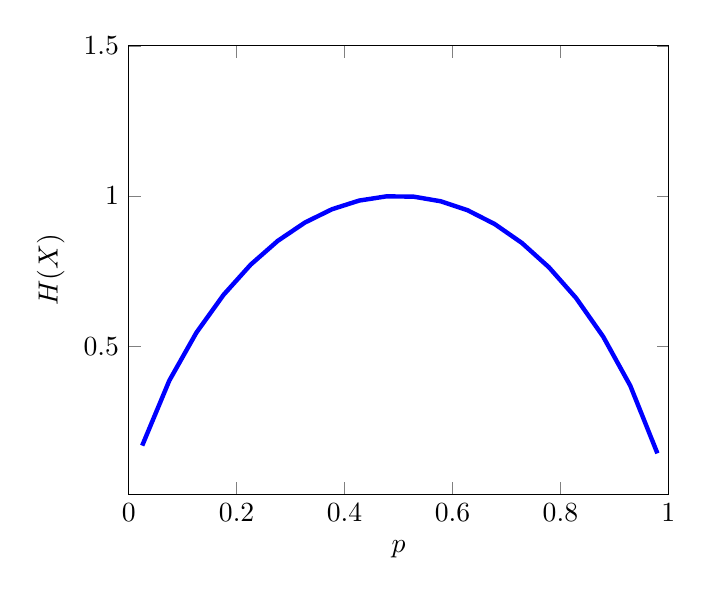
\begin{tikzpicture}
\begin{axis}[xmin=0, xmax=1 ,ymax=1.5, samples=50, xlabel = {$p$}, ylabel={$H(X)$}]
\addplot[blue, ultra thick, samples=200] (x, {x*log2((1-x)/x) - log2(1-x)});
\end{axis}
\end{tikzpicture}
\end{figure}

\begin{proposition}[Gibb's Inequality]
Let $(p_1, \ldots, p_n)$ and $(q_1, \ldots, q_n)$ be probability distributions. Then:
\begin{align*}
-\sum_{i=1}^n p_i \log p_i \leq -\sum_{i=1}^n p_i \log q_i
\end{align*}
with equality if and only if $p_i = q_i$ for all $i$.
\end{proposition}

\begin{proof}
Since $\log x = \frac{\ln x}{\ln 2}$, we may replace $\log$ by $\ln$ in the proof. Put $I = \{1 \leq r\leq n: p_i \neq 0\}$. Now $\ln x \leq x-1$ with equality if and only if $x=1$. So we have $\ln \frac{q_i}{p_i} \leq \frac{q_i}{p_i} - 1$, and hence:
\begin{align*}
\sum_{i \in I} p_i \ln \frac{q_i}{p_i} &\leq \sum_{i\in I}q_i - \sum_{i \in I}p_i\\
&= \sum_{i \in I} q_i - 1 \leq 0\\
\therefore - \sum_{i \in I}p_i \ln p_i &\leq - \sum_{i \in I} p_i \ln q_i\\
\therefore -\sum_{i=1}^n p_i \log p_i &\leq -\sum_{i=1}^n p_i \log q_i
\end{align*}
If equality holds, then $\sum_{i\in I} p_i =1$ and $\frac{p_i}{q_i} = 1$ for all $i \in I$, so $p_i = q_i$
\end{proof}

\begin{corollary}
$H(p_1, \ldots, p_n) \leq \log n$ with equality if and only if $p_1 = \ldots = p_n = \frac1n$.
\end{corollary}
\begin{proof}
Take $q_1 = \ldots = q_n = \frac1n$ in \textbf{2.1}.
\end{proof}

Let $\mathscr{A} = \{\mu_1, \ldots, \mu_m\}$, and $|\mathscr{B}| = a$, where $m, a\geq 2$. The random variable $X$ takes values $\mu_1, \ldots, \mu_m$ with probabilities $p_1, \ldots, p_m$. We say a code $c:\mathscr{A} \to \mathscr{B}^{\ast}$ is \emph{optimal} if it is a decipherable code with smallest possible expected word length, $\E S = \sum_i p_i \ell_i$.

\begin{theorem}[Shannon's Noiseless Coding Theorem]
The expected word length $\E S$ of an optimal code satisfies:
\begin{align*}
\frac{H(X)}{\log a} \leq \E S < \frac{H(X)}{\log a}+1
\end{align*}
\end{theorem}
\begin{proof}
For the lower bound, take $c: \mathscr{A} \to \mathscr{B}^{\ast}$ decipherable with word lengths $\ell_1, \ldots, \ell_m$. Then set $q_i = \frac{a^{-\ell_i}}{D}$ where $D = \sum_{i=1}^m a^{-\ell_i}$. Now we have that $\sum_{i=1}^m q_i = 1$. By Gibbs,
\begin{align*}
H(X) &\leq -\sum_{i=1}^m p_i \log q_i\\
&= -\sum p_i\left(-\ell_i \log a - \log D\right)\\
&= \left(\sum_{i=1}^m p_i \ell_i\right) \log a + \log D
\end{align*}
By McMillan, $D \leq 1$, so $\log D \leq 0$, and so $H(X) \leq \left(\sum_{i=1}^m p_i \ell_i\right) \log a = \E S \cdot \log a$, and we have equality if and only if $p_i = a^{-\ell_i}$ for some integers $\ell_1, \ldots \ell_m$.

For the upper bound, take $\ell_i = \ceil{-\log_a p_i}$. Then $-\log_a p_i \leq \ell_i \implies p_i \geq a^{-\ell_i}$.

Now $\sum_{i=1}^m a^{-\ell_i} \leq \sum_{i=1}^m p_i = 1$. By Kraft, there is some prefix-free code $c$ with word lengths $\ell_1, \ldots, \ell_m$, and the expected word length of $c$ is $\E S = \sum p_i \ell_i < \sum p_i (-\log_a p_i + 1) = \frac{H(X)}{\log a} + 1$.
\end{proof}

\hspace*{-1em}\underline{Example:} \emph{Shannon-Fano coding}\\
We mimic the above proof: given probabilities $p_1, \ldots, p_n$, set $\ell_i = \ceil{-\log_a p_i}$. Construct the prefix-free code with word lengths $\ell_1, \ldots, \ell_m$ by choosing in order of increasing length, ensuring that previous codewords are not prefixes. For example, if $a = 2, m = 5$ we have:\\
\begin{figure}[H]
\centering
\begin{tabular}{c|c|c|c}
$i$ & $p_i$ & $\ceil{-\log_2 p_i}$ & Codewords \\\hline
1 & 0.4 & 2 & 00 \\
2 & 0.2 & 3 & 010\\
3 & 0.2 & 3 & 011\\
4 & 0.1 & 4 & 1000\\
5 & 0.1 & 4 & 1001
\end{tabular}
\end{figure}
$\E S = \sum p_i \ell_i = 2.8$, entropy $= 2.12$

\section{Huffman Coding Algorithm}
Huffman was a student of Fano, and was thinking about how to construct an optimal code. For simplicity, we will take $a = 2$. Suppose we get messages with orders $p_1 \geq p_2 \geq \ldots \geq p_m$. Huffman gave a recursive definition of codes that we can prove are optimal. If $m=2$, then take codewords $0$ and $1$.

If $m > 2$, we first have a Huffman code for messages $\mu_1, \ldots, \mu_{m-2}, \nu$ with probabilities $p_1, \ldots, p_{m-2}, p_{m-1}+p_m$, then append $0$ and $1$ to give codewords for $\mu_{m-1}$ and $\mu_m$.

\hspace*{-1em}Note:
\begin{itemize}
\item Huffman codes are prefix-free.
\item We have some choices to make if some of the $p_j$ are equal, so Huffman codes are not unique.
\end{itemize}
\hspace*{-1em}\underline{Example:} Reconsider the previous example:
\begin{figure}[H]
\begin{subfigure}{0.5\textwidth}
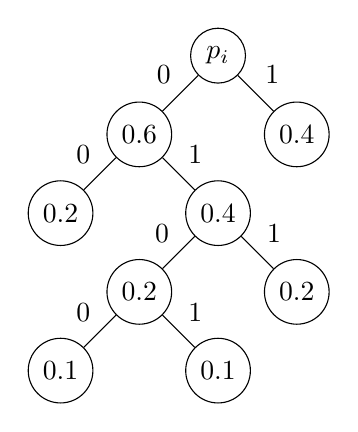
\begin{tikzpicture}
\node[draw, circle] (a) at (0,10) {$p_i$};
\node[draw, circle] (b) at (-1,9) {0.6};
\node[draw, circle] (c) at (1,9) {0.4};
\node[draw, circle] (d) at (0,8) {0.4};
\node[draw, circle] (e) at (-2,8) {0.2};
\node[draw, circle] (f) at (1,7) {0.2};
\node[draw, circle] (g) at (-1,7) {0.2};
\node[draw, circle] (h) at (0,6) {0.1};
\node[draw, circle] (i) at (-2,6) {0.1};

\draw (a) -- node[above left] {0} (b) (a) -- node[above right] {1} (c);
\draw (b) -- node[above left] {0} (e) (b) -- node[above right] {1} (d);
\draw (d) -- node[above left] {0} (g) (d) -- node[above right] {1} (f);
\draw (g) -- node[above left] {0} (i) (g) -- node[above right] {1} (h);
\end{tikzpicture}
\end{subfigure}
\begin{subfigure}{0.5\textwidth}
\begin{tabular}{c|c|c}
$i$ & $p_i$ & Codewords \\\hline
1 & 0.4 & 1\\
2 & 0.2 & 00\\
3 & 0.2 & 011\\
4 & 0.1 & 0100\\
5 & 0.1 & 0101
\end{tabular}
\end{subfigure}
\end{figure}
This code has expected length $2.2$, which is less than Shannon-Fano gave.
\begin{theorem}[Huffman, 1952]
Huffman codes are optimal.
\end{theorem}
\begin{proof}
We show this by induction on $m$. The case of $m=2$ is trivial. For $m > 2$, let $c_m$ be a Huffman code for source $X_m$ which takes values $\mu_1, \ldots, \mu_m$ with probabilities $p_1 \geq \ldots \geq p_m$. Then $c_{m-1}$ is constructed from a Huffman code $c_{m-1}$ for values $\mu_1, \ldots, \mu_{m-1}, \nu$ with probabilities $p_1, \ldots, p_{m-2}, p_{m-1}+p_m$.

Observe that $\E S_m = \E S_{m-1} + p_{m-1} + p_m$ by construction of $c_m$ from $c_{m-1}$.

Now let $c_m'$ be an optimal code for $X_m$. Without loss of generality, we may take $c_m'$ to be prefix-free and the last two codewords of $c_m'$ have maximal length and differ only in the last digit (see \textbf{3.2} below). Say $c_m'(\mu_{m-1}) = y0, c_m'(\mu_m) = y1$ for some $y \in \{0, 1\}^\ast$.

Let $c_{m-1}'$ be the prefix free code for $X_{m-1}$ given by $c_{m-1}'(\mu_i) = c_m'(\mu_i), c_{m-1}'(\nu) = y$.

Then the expected word length is $\E S_m' = \E S_{m-1}' + p_{m-1} + p_m \geq \E S_{m-1} + p_{m-1} + p_m = \E S_m$ by the inductive hypothesis, and so $c_m$ is optimal.
\end{proof}
\begin{lemma}
Suppose messages $\mu_1, \ldots, \mu_m$ are sent with probabilities $p_1,\ldots, p_m$, with an optimal code $c$ with word lengths $\ell_1, \ldots, \ell_m$. Then:
\begin{enumerate}
\item If $p_i > p_j$ then $\ell_i \leq \ell_j$.
\item Among all codewords of maximal length, there are two that differ only in the last digit.
\end{enumerate}
\end{lemma}
\begin{proof}
Otherwise, modify $c$ by swapping the $i\th$ and $j\th$ codewords, or deleting the last letter of each codeword of maximal length. The modified code is still prefix-free but has shorter expected word length, contradicting optimality of $c$.
\end{proof}
\section{Joint Entropy}
If $X,Y$ are random variables with value in $\mathscr{A}$ and $\mathscr{B}$. Then $(X,Y)$ is also a random variable with entropy $H(X,Y)$, the \emph{joint entropy} of $X,Y$.
\begin{align*}
H(X,Y) = -\sum_{x \in \mathscr{A}} \sum_{y \in \mathscr{B}} \P(X=x, Y=y)\log \P(X=x, Y=y)
\end{align*}
We can of course generalise this to any finite number of random variables. We will use Gibb's (\textbf{2.1}) to prove:
\begin{lemma}
Let $X,Y$ be random variables taking values in $\mathscr{A}, \mathscr{B}$. Then:\begin{align*}
H(X,Y) \leq H(X) + H(Y)
\end{align*}
with equality if and only if $X$ and $Y$ are independent.
\end{lemma}
\begin{proof}
Let $\mathscr{A} = \{x_1, \ldots, x_m\}, \mathscr{B} = \{y_1, \ldots, y_n\}$. Set $p_{ij} = \P(X=x_i, Y=y_i), p_i = \P(X=x_i), q_i = \P(Y=y_i)$. Then Gibb's inequality with $\{p_{ij}\}$ and $\{p_iq_j\}$ gives:
\begin{align*}
-\sum_{i,j} p_{ij}\log p_{ij} \leq -\sum_{i,j} p_{ij}\log(p_iq_j) &= -\sum_i\left(\sum_j p_{ij}\right) \log p_i - \sum_j \left(\sum_i p_{ij}\right) \log q_j\\
&= -\sum_i p_i \log p_i -\sum_j q_j \log q_j
\end{align*}
i.e. $H(X,Y) \leq H(X) + H(Y)$, with equality if and only if $p_{ij} = p_i q_j$ for all $i, j$, i.e. when $X,Y$ are independent.
\end{proof}

\hspace*{-1em}\underline{Example:} Let $X$ be a random variable that takes $D$ values with probability $\frac1D$. Then $H(X) = \log_2(D)$. Suppose $X_1, \ldots, X_N$ are i.i.d. with the same distribution as $X$. Then $H(X_1, \ldots, X_N) = N \log_2 D$.

\section{Error Correcting Codes}
\subsection{Noisy Channels and Hamming's Code}
A \emph{binary [n,m]-code} is a subset $C \subseteq \{0,1\}^n$ of \emph{size} $m = |C|$, \emph{length} $n$. The elements of $C$ are called \emph{codewords}. We use an $[n,m]$-code to send one of $m$ messages through a binary symmetric channel, making $n$ uses of the channel. Clearly $1 \leq m \leq 2^n$, so $0\leq \frac{1}{n}\log m \leq 1$. If $|C| = 1$ then $\rho(C) = 0$, and if $C= \{0,1\}^n$ then $\rho(C) = 1$.

For $x, y \in \{0,1\}^n$, the \emph{Hamming distance} $d(x,y) = |\{i:1\leq i\leq n, x_i \neq y_i \}|$, i.e. the number of positions where $x$ and $y$ differ.

We have three possible decoding rules:
\begin{enumerate}
\item The \emph{ideal observer} decoding rule decodes $x \in \{0,1\}^n$ as $c\in C$ maximising $\P(c$ sent$|x$ received$)$.
\item Then \emph{maximum likelihood} decoding rule decodes $x \in \{0,1\}^n$ as $c\in C$ maximising $\P(x$ received$|c$ sent$)$.
\item The \emph{minimum distance} decoding rule decodes $x \in \{0,1\}^n$ as $c\in C$ minimising $d(x,c)$.
\end{enumerate}

\begin{lemma}
\item
\begin{enumerate}
\item If all the messages are equally likely, then 1. and 2. agree.
\item If $p < \frac{1}{2}$, then 2. and 3. agree.
\end{enumerate}
\end{lemma}
\begin{proof}
\item
\begin{enumerate}
\item By Bayes' Rule:
\begin{align*}
\P(c\sent |x \received) = \frac{\P(c \sent)}{\P(x\received)}\P(x\received|c\sent)
\end{align*}
\end{enumerate}
By Hypothesis, $\P(c\sent)$ is independent of $c \in C$, and so for fixed $x$, maximising $\P(c\sent|x\received)$ is the same as maximising $\P(x\received|c\sent)$.

\item Let $r = d(x,c)$. Then $\P(x\received|c\sent) = p^r(1-p)^{n-r} = (1-p)^n\left(\frac{p}{1-p}\right)^r$. Since $p < \frac12$, $\frac{p}{1-p} < 1$, and so maximising $\P(x\received|c\sent)$ is the same as minimising $d(x, c)$.
\end{proof}

For instance, suppose $000$ is sent with probability $\frac{9}{10}$, and $111$ with probability $\frac{1}{10}$, through a binary symmetric channel with error probability $\frac14$. If we receive $110$, the ideal receiver computes $\P(000\sent|110\received)=\frac34; \P(110\sent|110\received)=\frac14$, and so decodes it as $000$. But the minimum distance (and so maximal likelihood) code is $111$. Henceforth, we will decide to use minimal distance decoding. 

Note that minimal distance decoding can be expensive in terms of time and storage if $|C$ is large, and we also need to specify a convention in the case of a tie (e.g. make a random choice, request the message again).

A code is \emph{d-error detecting} if changing up to $d$ digits in each codeword can never produce another codeword. It is \emph{e-error correcting} if, knowing that $x \in \{0,1\}^n$ differs from some codeword in at most $e$ places, we can deduce uniquely what the codeword is.

\hspace*{-1em}\underline{Examples}
\begin{enumerate}
\item A \emph{repetition code} of length $n$ has codewords $00\ldots0, 11\ldots1$. This is an $[n,2]$-code. It is $(n-1)$ error detecting and $\floor{\frac{n-1}{2}}$-error correcting. But the information rate is only $\frac1n$.
\item A \emph{simple parity check code} or \emph{paper tape code}: identify $\{0,1\}$ with $\F_2$ (i.e. arithmetic modulo 2), and let $C = \{(x_1,\ldots, x_n)\in \{0,1\}^n : \sum x_i = 0\}$. This is an $[n, 2^{n-1}]$-code. It is 1-error detecting, but cannot correct errors. Its information rate is $\frac{n-1}{n}$.
\item \emph{Hamming's Original Code} is a $2$-error detecting and 1-error correcting binary [7,16]-code:
\begin{align*}
C = \left.\begin{cases} & c_1+c_3+c_5+c_7 = 0\\ c \in \F_2^7 : & c_2+c_3+c_6+c_7 = 0\\ &c_4+c_5+c_6+c_7 = 0\end{cases}\right\}
\end{align*}
\end{enumerate}
The bits $c_3,c_5,c_6,c_7$ are arbitrary and $c_1, c_2, c_4$ are forced. The information rate is $\frac47$.

Given $x \in \F_2^7$, we form the \emph{syndrome} $z = (z_1,z_2,z_4) \in \F_2^7$, where $z_1 = x_1+x_3+x_5+x_7,$ $z_2 = x_2+x_3+x_6+x_7,$ $z_4 = x_4+x_5+x_6+x_7$. If $x \in C$ then $z = (0,0,0)$. If $d(x,c) = 1$ for some $c \in C$ then $x_i$ and $c_i$ differ for $i = z_1 + 2z_2 + 4z_4$. This can be checked easily for $c=0$ with a case by case check of the seven binary sequences of six 0s and one 1, e.g. $x=0010000$ gives a syndrome $z = (1,1,0), i = 1+2+0 = 3$.

\begin{lemma}
$d$ is a metric on $\F_2^n$.
\end{lemma}
\begin{proof}
Immediately, $d(x,y) \geq 0$, with equality if and only if $x=y$, and $d(x,y)=d(y,x)$. For the triangle inequality, note that if $x$ and $z$ differ at position $i$ then either $x,y$ differ at $i$ or $y,z$ differ at $i$. So every difference appearing in $d(x,z)$ appears in $d(x,y)+d(y,z)$, so $d(x,z) \leq d(x,y)+d(y,z)$.
\end{proof}

Note that $d(x,y) = \sum_i d_1(x_i,y_i)$ where $d_1$ is the discrete metric on $\F_2$. We define the \emph{minimum distance} of a code to be $\min_{c_1 \neq c_2} d(c_1,c_2)$.

\begin{lemma}
Let $C$ have minimal distance $d$. Then:
\begin{enumerate}
\item $C$ is $(d-1)$-error detecting, but cannot detect all sets of $d$ errors.
\item $C$ is $\floor{\frac{d-1}{2}}$-error correcting, but cannot correct all sets of $\floor{\frac{d-1}{2}}+1$ errors.
\end{enumerate}
\end{lemma}
\begin{proof}
\item
\begin{enumerate}
\item $d(c_1,c_2) \geq d$ for all distinct $c_1, c_2 \in C$. So $C$ is $(d-1)$-error detecting. But $d(c_1, c_2)=d$ for some $c_1, c_2 \in C$. So $C$ cannot detect all sets of errors.

\item Define the closed Hamming ball with center $x \in \F_2^n$, radius $r\geq 0$ as $B(x,r) = \{y \in \F_2^n: d(x,y)\leq r\}$. Now $C$ is $e$-error correcting if and only if, for all $c_1 \neq c_2 \in C$, we have $B(c_1, e) \cap B(c_2, e) = \emptyset$.

If $x \in B(c_1,e) \cap B(c_2,e )$, then $d(c_1,c_2) \leq d(c_1,x)+d(x,c_2) \leq 2e$. So if $d \geq 2e+1$, then $C$ is $e$-error correcting, with $e = \floor{\frac{d-1}{2}}$. For the second part, take $c_1, c_2 \in C$ with $d(c_1, c_2) = d$. Then suppose $x \in \F_2^n$ differs from $c_1$ in $e$ digits where $c_1, c_2$ differ too. Then $d(x,c_1) = e, d(x,c_2) = d-e$. If $d < 2e$ then $B(c_1, e) \cap B(c_2, d-e) \neq 0$, and so $C$ cannot correct all sets of $e$-errors. Then take $e = \ceil{\frac{d}{2}} = \floor{d-1}{2}+1$.
\end{enumerate}
\end{proof}
As a point of a notation, an $[n,m]$-code with minimum distance $d$ will be denoted as an $[n,m,d]$-code.

\hspace*{-1em}\underline{Examples:}
\begin{enumerate}
\item Repetition of length $n$ is an $[n,2,n]$-code.
\item Simple parity check code of length $n$ is an $[n, 2^{n-1}, 2]$-code.
\item Hamming's code is 1-error correcting, so $d\geq 3$. 0000000, 1110000 are both codewords, so it is a $[7,16,3]$-code, and hence 2-error correcting.
\end{enumerate}

\section{Covering Estimates}
Denote $V(n,r) = |B(x,r)| = \sum_{i=0}^r \binom{n}{i}$, independent of $x \in \F_2^n$, as the \emph{volume} of the ball (i.e. the number of points it contains).

\begin{lemma}[Hamming's Bound]
An $e$-error correcting code of length $n$ has:
\begin{align*}
|C| \leq \frac{2^n}{V(n,e)}
\end{align*}
\end{lemma}
\begin{proof}
Suppose $C$ is $e$-error correcting. Then $B(c_1, e) \cap B(c_2, e) = \emptyset$ for all $c_1 \neq c_2 \in C$. Then $\sum_{c \in C} |B(c,e)| \leq |\F_2^n| = 2^n$, i.e. $|C|V(n,e) \leq 2^n$.
\end{proof}
A code $C$ of length $n$ that can correct $e$ errors is \emph{perfect} if $|C|=\frac{2^n}{V(n,e)}$. Equivalently, a code is perfect if for all $x \in \F_2^n$ there is a unique $c \in C$ such that $d(x,c) \leq e$, or $\F_2^n = \bigcup_{c\in C}B(c,e)$, i.e. any $e+1$ errors will make you decode incorrectly.

For example, Hamming's $[7,16,3]$-code is perfect, as $\frac{2^7}{7+1} = 2^4 = |C|$. Note that if $\frac{2^n}{V(n,e)} \notin \Z$ then there is no perfect $e$-error correcting code of length $n$, and even if $2^n/V(n,e)$ is an integer is may be the case that no perfect code exists.

Define \emph{A(n,d)} $= \max\{m : \exists [n,m,d]$-code$\}$. For instance, $A(n,1) = 2^n, A(n,n) = 2, A(n,2) = 2^{n-1}$.

\begin{lemma}
$A(n,d+1) \leq A(n,d)$
\end{lemma}
\begin{proof}
Let $m = A(n,d+1)$, and pick a code $C$ with parameters $[n,m,d+1]$. Let $c_1, c_2 \in C$ with $d(c_1,c_2) = d+1$. Let $c_1'$ differ from $c_1$ in exactly one of the places where $c_1, c_2$ differ. Then $d(c_1', c_2) = d$. If $c \in C\setminus\{c_1\}$, then $d(c,c_1)\leq d(c,c_1')+d(c_1', c_1) \implies d(c_1, c_1') \geq d$.

Replacing $c_1$ by $c_1'$ gives an $[n,m,d]$-code i.e. $m \leq A(n,d)$.
\end{proof}

\begin{corollary}
Equivalently, $A(n,d) = \max\{m : \exists [n,m,d']-$code for some $d'\geq d\}$.
\end{corollary}
\begin{theorem}
\begin{align*}
\frac{2^n}{V(n,d-1)} \leq A(n,d) \leq \frac{2^n}{V(n, \floor{\frac{d-1}{2}})}
\end{align*}
The lower bound is called the Gilbert-Shannon-Varshanov (GSV) bound, whilst the upper bound follows from Hamming's bound.
\end{theorem}
\begin{proof}[Proof of GSV]
Let $m = A(n,d)$, and let $C$ be a $[n,m,d]$-code. Then there cannot exist $x \in \F_2^n$ with $d(x,c) \geq d$ for all $c \in C$, otherwise we could replace $C$ by $C \cup \{x\}$, contradicting maximality of $d(x,c)$. Hence $\F_2^n = \bigcup_{c\in C} B(c, d-1)$. Hence $2^n \leq m V(n, d-1)$.
\end{proof}
For example, take $n=10, d=3$. Then $V(n,2) = 56, V(n,1)=11$, and so these bounds give $\frac{2^10}{56} \leq A(10,3) \leq \frac{2^10}{11}$, i.e. $19\leq A(10,3)\leq 93$, but in fact we know computationally that it is between 72 and 79.

\subsection{Asymptotics}
We study $\frac{\log A(n, \floor{n\delta})}{n}$ as $n \to \infty$ to see how large the information rate can be for a given error rate.
\begin{proposition}
Let $0 < \delta < \frac12$. Then:
\begin{enumerate}
\item $\log V(n, \floor{n \delta}) \leq n H(\delta)$.
\item $\frac1n \log A(n, \floor{n\delta}) \geq 1- H(\delta)$.
\end{enumerate}
\end{proposition}
\begin{proof}
Assuming \textit{1.} we see by the GSV bound, $A(n, \floor{n\delta}) \geq \frac{2}{V(n, \floor{n\delta}-1} \geq \frac{2^n}{V(n, \floor{n\delta})}$, so $\frac{\log A(n, \floor{n\delta})}{n} \geq 1 - \frac{\log V(n, \floor{n\delta})}{n} \geq 1- H(\delta)$, and so \textit{1.}$\implies$\textit{2.}

For \textit{1.} observe $H(\delta)$ is increasing for $\delta \leq \frac12$, so \textsc{wlog} we can assume $n\delta \in \Z$. Then:
\begin{align*}
1 &= (\delta + (1-\delta))^n\\
&= \sum_{i=0}^n \binom{n}{i} \delta^i (1-\delta)^{n-i}\\
&\geq \sum_{i=0}^{n\delta} \binom{n}{i} \delta^i (1-\delta)^{n-i}\\
&= (1-\delta)^n \sum_{i=0}^{n\delta} \binom{n}{i} \left(\frac{\delta}{1-\delta}\right)^i\\
&\geq (1-\delta)^n \sum \binom{n}{i} \left(\frac{\delta}{1-\delta}\right)^{n\delta}\\
&= \delta^{n\delta}(1-\delta)^{n(1-\delta)}V(n,n\delta)\\
0 &\geq n\delta\log\delta + n(1-\delta)\log(1-\delta)+\log V(n,n\delta)\\
0 &\geq -nH(\delta) + \log V(n,n\delta)
\end{align*}
\end{proof}
This constant $H(\delta)$ is the best possible, in the sense that:
\begin{proposition}
\begin{align*}
\lim_{n\to\infty} \frac{\log V(n, \floor{n\delta})}{n} = H(\delta)
\end{align*}
\end{proposition}
\begin{proof}
\textsc{Wlog} we may assume that $0 < \delta < \frac12$. Let $0 \leq r \leq \frac{n}{2}$. Recall that $V(n,r) = \sum_{i=0}^r \binom{n}{i}$. Then:
\begin{align*}
\binom{n}{r} \leq V(n,r) \leq (r+1)\binom{n}{r} \tag{(\ast)}
\end{align*}
From Stirling's approximation, $\log\binom{n}{r} = -r\log \frac{r}{n} - (n-r)\log\frac{n-r}{n} + \mathcal{O}(\log n) = nH(\frac{r}{n}) + \mathcal{O}(\log n)$.

Then from $(\ast)$, we have:
\begin{align*}
H(\frac{r}{n}) + \mathcal{O}\left(\frac{\log n}{r}\right) \leq \frac{\log V(n,r)}{n} \leq H\left(\frac{r}{n}\right) + \mathcal{O}\left(\frac{\log n}{n}\right)\\
\therefore \lim_{n\to\infty} \frac{\log V(n, \floor{n\delta})}{n} = H(\delta)
\end{align*}
\end{proof}
\section{New Codes from Old}
Suppose $C$ is an $[n,m,d]$-code. Then the \emph{parity check digit extension} $C^+$ of $C$ is the code of length $n+1$ given by:
\begin{align*}
C^+ = \{(c_1, \ldots, c_n, \sum_{i=1}^n c_i) : (c_1, \ldots, c_n) \in C\}
\end{align*}
where the summation is done modulo 2. It is an $[n+1, m, d']$-code where $d' = d$ or $d+1$.

We can also delete the $i\th$ digit from each codeword for $1 \leq i\leq n$, giving a \emph{truncated} or \emph{punctured} codeword (depending on if $i=n$ or $i<n$ respectively), called $C^-$, with parameters $[n-1, m, d']$ where $d-1 \leq d' \leq d$.

Finally, given some $1 \leq i \leq n, \alpha \in \F_2$, we can create the \emph{shortened} or \emph{punctured} code $C'$ of $C$ is $\{(c_1, \ldots, c_{i-1},c_{i+1}, \ldots, c_n) : (c_1, \ldots, c_{i-1}, \alpha, c_{i+1} \ldots, c_n) \in C\}$. This has parameters $[n-1, m', d']$ with $d' \geq d$ and $m' \geq \frac{m}{2}$ for $c$ a suitable choice of $\alpha$.

\section{AEP and Shannon's First Coding Theorem}
A \emph{source} is a sequence of random variables $X_1, X_2, \ldots$ taking values in some alphabet $\mathscr{A}$. A source is \emph{Bernoulli} or \emph{memoryless} if $X_1, \ldots$ are independently identically distributed (\textsc{iid}). A source $X_1, \ldots$ is \emph{reliably encodable at rate r} if there are subsets $A_n \subseteq \mathscr{A}^n$ such that:
\begin{enumerate}
\item $\lim_{n\to \infty} \frac{\log|A_n|}{n} = r$
\item $\lim_{n\to \infty} \P[(X_1, \ldots, X_n)\in A_n] = 1$
\end{enumerate}
The \emph{information rate} $H$ of a source is the infimum of all reliable encoding ratesso that $0 \leq H \leq \log |\mathscr{A}|$. Shannon's first coding theorem computes the information rate of certain sources, including Bernoulli sources.

\subsection{Reminder from 1A Probability}
A \emph{probability space} is given by a triple $(\Omega, \mathscr{F}, \P)$ where $\mathscr{F} \subset \powset(\Omega)$ is a set of \emph{events} and $\P$ is a \emph{probability measure}, and a \emph{random variable} $X$ is a function defined on $\Omega$ with some range. It has a \emph{probability mass function} $p: x \mapsto \P(X=x)$

We say that a sequence of random variables $X_1, X_2, \ldots$ \emph{converges in probability} to $\lambda \in \R$ means that
\begin{align*}
\forall\;\epsilon > 0, \lim_{n \to \infty} \P(|X_n -\lambda| \geq \epsilon) = 0
\end{align*}
We write $X_n \xrightarrow{\P} \lambda$ as $n \to \infty$.

\begin{theorem}[Weak Law Of Large Numbers, \textsc{wlln}]
Let $X_1, X_2, \ldots$ be \textsc{iid} discrete real-valued random variables with finite expected value $\mu$. Then:
\begin{align*}
\frac1n \sum_{i=1}^n X_i \xrightarrow{\P} \mu\text{ as } n\to \infty
\end{align*}
\end{theorem}
\begin{proof}
See Carne, theorem 10.3.
\end{proof}
\begin{lemma}
The information rate of a Bernoulli source $X_1, X_2, \ldots$ is at most the expected word length of an optimal code $c:\mathscr{A} \to \{0,1\}^{\ast}$ for $X_i$.
\end{lemma}
\begin{proof}
Let $\ell_1, \ell_2, \ldots$ be the lengths of codewords when we encode $X_1, X_2, \ldots$ using $c$. Then given $\epsilon >0$, let $A_n = \{x \in \mathscr{A}^n : c^{\ast}(x)$ has length $< n(\E[\ell_i] + \epsilon)\}$. Then:
\begin{align*}
\P\left[(X_1, \ldots, X_n) \in A_n\right] &= \P\left[\sum \ell_i < n(\E[\ell_i] +\epsilon)\right]\\
&\geq \P\left(\left|\frac1n \sum\ell_i - \E[\ell_i]\right| < \epsilon\right)\\
&\to 1 \text{ as } n \to \infty
\end{align*}
Now $c$ is decipherable so $c^{\ast}$ is injective, and hence $|A_n| \leq 2^{n(\E[\ell_i]+\epsilon)}$. Making $A_n$ larger if required, we may take $|A_n| =\floor{2^{n(\E[\ell_i]+\epsilon)}}$. Hence $\frac{\log|A_n|}{n} \to \E[\ell_i] + \epsilon$. So $X_1, X_2, \ldots$ is reliably encodable at a rate $r = \E[\ell_i] +\epsilon$ for any $\epsilon > 0$, and hence the information rate is at most $\E[\ell_i]$.
\end{proof}
\begin{corollary}
A Bernoulli source has information rate less than $H(X_1) + 1$.
\end{corollary}
\begin{proof}
Use \textbf{8.2} and the Noiseless Coding theorem \textbf{2.3}.
\end{proof}

Now suppose we encode $X_1, X_2, \ldots$ in blocks:
\begin{align*}
\underbrace{X_1, \ldots, X_N}_{Y_1}, \underbrace{X_{N+1}, \ldots, X_{2N}}_{Y_2}, \ldots
\end{align*}
such that $Y_1, Y_2, \ldots$ take values in $\mathscr{A}^N$. We can check that if $X_1,  X_2, \ldots$ has information rate $H$, then $Y_1, Y_2, \ldots$ has information rate $NH$.

\begin{proposition}
The information rate$H$ of a Bernoulli source $X_1, X_2, \ldots$ is at most $H(X_1)$.
\end{proposition}
\begin{proof}
Apply \textbf{8.3} to $Y_1, Y_2, \ldots$ to get:
\begin{align*}
NH < H(Y_1) + 1 = H(X_1, \ldots, X_N) + 1 = \sum_{i=1}^N H(X_i) + 1 = NH(X_i)+1
\end{align*}
i.e. $H < H(X_1) + \frac1N$ for all $N \geq 1$, and so $H \leq H(X_1)$.
\end{proof}

\hrule
\subsection{Typical Sequences}
This content is nonexaminable, but is required to prove the examinable result that $H = H(X_1)$.

\hspace*{-1em}As a motivational example, toss a biased coin with head probability $p$, and let $X_i$ be the outcome of the $i\th$ flip. If we toss a large number, say $N$, times, we expect that we will get about $pN$ heads and $(1-p)N$ tails. The probability of any particular sequence of $pN$ heads and $(1-p)N$ tails is $p^{pN}(1-p)^{(1-p)N} = 2^{-NH(X)}$.

We say that a source $X_1, X_2, \ldots$ satisfies the \emph{Asymptotic Equipartition Property (AEP)} for some constant $H \geq 0$ if:
\begin{align*}
-\frac1n\log p(X_1, \ldots, X_n) \to H \text{ as } n \to \infty
\end{align*}
\begin{lemma}
The AEP for a source $X_1, x_2, \ldots$ is equivalent to the following:\\
$\forall\;\epsilon>0 \exists n_0(\epsilon) \st \forall\;n\geq n_0(\epsilon) \exists T_n \subseteq \mathscr{A}^n \st$
\begin{itemize}
\item $P[(X_1, \ldots, X_n) \in T_n] > 1-\epsilon$
\item $\forall\;(x_1, \ldots, x_n) \in T_n, 2^{-n(H+\epsilon)} \leq p(x_1, \ldots, x_n) \leq 2^{-n(H-\epsilon)}$
\end{itemize}
The $T_n$ are called \emph{typical sets}, and the $(x_1, \ldots, x_n) \in T_n$ are \emph{typical sequences}.
\end{lemma}
\begin{proof}
If $(x_1, \ldots, x_n) \in \mathscr{A}^n$ then we have the following equivalence:
\begin{align*}
2^{-n(H+\epsilon)} \leq p(x_1, \ldots, x_n) \leq 2^{-n(H-\epsilon)} \iff |-\frac1n \log p(x_1, \ldots, x_n) - H| \leq \epsilon \tag{\dagger}
\end{align*}
Both AEP and the claimed equivalent results say that $P((X_1, \ldots, X_N)\text{ satisfies } \dagger) \to 1$ as $n \to \infty$.
\end{proof}

\begin{theorem}[Shannon's First Coding Theorem]
If a source $X_1, X_2, \ldots$ satisfies the AEP with constant $H$ then it has information rate $H$.
\end{theorem}
\begin{proof}
Let $\epsilon >0$ and let $T_n \subseteq \mathscr{A}^n$ be typical sets. Then for all $(x_1, \ldots, x_n) \in T_n$:
\begin{align*}
p(x_1, \ldots, x_n) \geq 2^{-n(H+\epsilon)} \implies 1 \geq |T_n|2^{-n(H+\epsilon)} \implies \frac{\log|T_n|}{n} \leq (H+\epsilon)
\end{align*}
Taking $A_n = T_n$ in the definition of reliable encoding, we see that the source is reliably encodeable at rate $H+\epsilon$. As $\epsilon >0$, the information rate is $\leq H$.

Conversely, if $H=0$ we're done, otherwise pick $0 <\epsilon < \frac{H}{2}$. Suppose for a contradiction that the source is reliably encodeable at rate $H-2\epsilon$, say, with sets $A_n \subseteq \mathscr{A}^n$. Let $T_n \subseteq \mathscr{A}^n$ be typical sets. Then for all $(x_1, \ldots, x_n) \in T_n, p(x_1, \ldots, x_n) \leq 2^{-n(H-\epsilon)}$

Hence $\P(A_n \cap T_n) \leq 2^{-n(H-\epsilon)}$, and so $\frac{\log\P(A_n\cap T_n)}{n} \leq (H-\epsilon) + \frac{\log |A_n|}{n}\xrightarrow{n \to \infty} -\epsilon$. So $\P(A_n \cap T_n) \to 0$ as $n \to \infty$. But $\P(T_n) \leq \P(T_n\cap A_n) + \P(\mathscr{A}^n \setminus A_n) \to 0 + 0 = 0$ as $n \to \infty$, contradicting typicality of $T_n$. Hence the source cannot be reliably encoded at rate $H-2\epsilon$, and so the information rate must be $\geq H$, and hence $=H$.
\end{proof}
\section{Capacity and Shannon's Second Coding Theorem}
Given a random variable $X$ with mass function $p_X$, we can construct a new random variable $p(X) = p_X \circ X$, taking values in $[0,1]$. Then $H(X) = \E(-\log p(X))$. For example, if $X,Y$ are independent, then $p(X,Y) = p(X)p(Y)$, and so $-\log p(X,Y) = -\log p(X) - \log p(Y) \implies H(X,Y) = H(X)+H(Y)$.

\begin{corollary}
A Bernoulli source $X_1, X_2, \ldots$ has information rate $H(X_1) = H$.
\end{corollary}
\begin{proof}[Proof*]
$p(X_1, \ldots, X_n) = p(X_1)\ldots p(X_n)$, and hence we have:
\begin{align*}
-\frac{\log p(X_1, \ldots X_n)}{n} = -\frac{1}{n}\sum_{i=1}^n \log p(X_i) \xrightarrow{\P} H(X_i)
\end{align*}
by the weak law of large numbers, and using the fact that the $X_i$ are i.i.d. Check as an exercise that the AE holds with constant $H(X_1)$ using the definition of convergence in probability. Hence by \textbf{8.6} we are done.
\end{proof}
Note that \textbf{8.4} gave us an information rate $\leq H(X_1)$, without the use of the AEP. The AEP can also be used for noiseless coding - we encode the typical sequences with a block code and the atypical sequences arbitrarily, since they rarely occur. Many sources of interest, not just Bernoulli sources, satisfy the AEP. Under suitable conditions, the sequence $\frac1n H(X_1, \ldots, X_n)$ is decreasing and the AEP is satisfied with constant $H \lim_{n\to \infty} \frac{H(X_1,\ldots, X_n}{n}$.

Consider a communication channel with input of alphabet $\mathscr{A}$, and output $B$. A code of length $n$ is a subset $C \subseteq \mathscr{A}^n$. The \emph{error rate}
\begin{align*}
\hat{e}(C) = \max \P(\text{error }|c\text{ sent})
\end{align*}

The \emph{information rate} is $\rho(C) = \frac{\log |C|}{n}$.

The channel can \emph{transmit reliably} at rate $R$ if there are codes $C_1, C_2, \ldots$ with $C_n$ of length $n$, and:
\begin{itemize}
\item $\lim_{n \to \infty} \rho(C_n) = R$.
\item $\lim_{n \to \infty} \hat{e}(C_n) = 0$.
\end{itemize}
The \emph{operational capacity} is the supremum of all reliable transmission rates.

Assume a source has information rate $r$ bits per symbol, and emits symbols at $s$ symbols per second, whilst the channel has capacity $R$ bits per transmission and can can transmit symbols at $S$ transmissions per second. Usually $S=s=1$. If $rs \leq RS$ then we can encode and transmit reliably, and if $rs > RS$ we cannot.

\begin{proposition}
A binary symmetric channel with error probability $p < \frac{1}{4}$ has non-zero capacity.
\end{proposition}
\begin{proof}
We use the $GSV$ bound. Pick $\delta$ with $2p <\delta  < \frac12$. We claim reliable transmission rate of $R = 1-H(\delta) > 0$.

Let $C_n$ be a code of length $n$ with minimum distance $\floor{n\delta}$ of maximal size. Them $|C_n| = A(n, \floor{n\delta}) \geq 2^{n(1-H(\delta)} = 2^{nR}$.

Replacing $C_n$ by a subcode we can assume $|C_n| = \floor{2^{nR}}$ with minimum distance still $\geq \floor{n\delta}$

Now, with minimum distance decoding, $\hat{e}(C_n) \leq \P($in $n$ uses the BSC makes more than $\frac{n\delta-1}{2}$ errors$)$.

Pick $\epsilon > 0$ with $p+\epsilon < \frac{\delta}{2}$. For $n$ sufficiently large we have that $\frac{n\delta-1}{2} = n(\frac{\delta}{2} - \frac{1}{2n}) > n(p+\epsilon)$.

Hence $\hat{e}(C) \leq \P($BSC makes more than $n(p+\epsilon)$ errors$) \to 0$, as we will see in the next lemma.
\end{proof}
\begin{lemma}
Let $\epsilon > 0$. A BSC with error probability $p$ is used to transmit $n$ digits. Then:
\begin{align*}
\lim_{n \to \infty} \P(\text{BSC makes at least }n(p+\epsilon)\text{ errors}) = 0
\end{align*}
\end{lemma}
\begin{proof}
If $U_i$ is the Bernoulli random variable that digit $i$ is mistransmitted. Then $U_i$ are i.i.d. with probability $p$. So $\E[U_i] = p$. Then the probability we are interested in is $\P(\sum U_i \geq n(p+\epsilon)) \leq \P(|\frac{1}{n}\sum U_i -p| \geq \epsilon) \to 0$ by the \textsc{wlln}.
\end{proof}

\subsection{Fano's Inequality}
Let $X,Y$ be random variables taking values in the alphabets $\mathscr{A}, \mathscr{B}$. Then:
\begin{itemize}
\item $H(X|Y=y) = -\sum_{x \in \mathscr{A}} \P(X=x|Y=y)\log \P(X=x|Y=y)$
\item $H(X|Y) = \sum_{y \in \mathscr{B}} \P(Y=y)H(X|Y=y)$
\end{itemize}
Clearly $H(X|Y) \geq 0$.
\begin{lemma}
\begin{align*}
H(X,Y) = H(X|Y) + H(Y)
\end{align*}
\end{lemma}
\begin{proof}
\begin{align*}
H(X|Y) &= -\sum_{x\in\mathscr{A}} \sum_{y \in \mathscr{B}} \P(X=x|Y=y)\P(Y=y)\log \P(X-x|Y=y)\\
&= -\sum_{x\in\mathscr{A}} \P(X=x, Y=y) \log \frac{\P(X=x, Y=y}{\P(Y=y)}\\
&= -\sum_{(x,y)\in\mathscr{A}\times\mathscr{B}}\underbrace{\P(X=x,Y=y)\log\P(X=x,Y=y)}_{H(X,Y)} + \underbrace{\P(X=x, Y=y)\log\P(Y=y)}_{-H(Y)}\\
&= H(X,Y) - H(Y)
\end{align*}
\end{proof}
\begin{corollary}
$H(X|Y) \leq H(X)$ with equality if and only if $X,Y$ are independent.
\end{corollary}
\begin{proof}
Combine \textbf{4.1} with \textbf{9.4}.
\end{proof}
We can replace $X,Y$ by random variables $X_1, X_2, \ldots, X_r$ and $Y_1, Y_2, \ldots, Y_s$, and similarly define $H(X_1, \ldots, X_r|Y_1, \ldots, Y_s)$\footnote{$H(X,Y|Z)$ means ``the entropy of ($X$ and $Y$) given $Z$", \textsc{not} ``the entropy of $X$ and ($Y$ given $Z$)"}.

\begin{lemma}
\begin{align*}
H(X|Y) \leq H(X|Y, Z) + H(Z)
\end{align*}
\end{lemma}
\begin{proof}
\begin{align*}
H(X,Y,Z) &= H(Z|X,Y) + H(X,Y) = H(Z | X, Y) + H(X|Y) + H(Y)\\
H(X,Y,Z) &= H(X|Y,Z) + H(Y,Z) = H(X|Y, Z) + H(Z|Y) + H(Y)\\
\therefore H(X|Y) &= -H(Z|X,Y) + H(X|Y,Z) + H(Z|Y)\\
&\leq H(X|Y,Z) + H(Z) 
\end{align*}
\end{proof}
\begin{proposition}[Fano's Inequality]
Let $X,Y$ be random variables taking values in $\mathscr{A}$, where $|\mathscr{A}| = m$. Let $p = \P(X\neq Y)$. Then:
\begin{align*}
H(X|Y) \leq H(p) + p \log(m-1)
\end{align*}
\end{proposition}
\begin{proof}
Let $Z = \begin{cases} 0 & X = Y \\ 1 & X \neq Y\end{cases}$. Then $\P(Z=0) = 1-p, \P(Z=1) = p$. So $H(Z) = H(p)$. By \textbf{9.6},
\begin{align*}
H(X|Y) \leq H(p) + H(X|Y,Z)\tag{\ast}
\end{align*}
Then we have two cases:
\begin{itemize}
\item[$Z=0$:] We must have $X=y$, so $H(X|Y=y, Z=0) = 0$.
\item[$Z=1$:] Just $m-1$ remaining possibilities for $X$, so $H(X|Y=y, Z=1) \leq \log(m-1)$.
\end{itemize}
Hence we have:
\begin{align*}
H(X|Y,Z) &= \sum_{y,z} \P(Y=y, Z=z)H(X|Y=y,Z=z)\\
&\leq \sum_y \P(Y=y, Z=1)\log(m-1)\\
&= \P(Z=1)\log(m-1) = p\log(m-1)
\end{align*}
Then by $(\ast)$, $H(X|Y) \leq H(p) + p \log(m-1)$.
\end{proof}
We will apply this result later when $X$ takes values in $\mathscr{A}$ and $Y$ is the result of passing codewords through a channel and then decoding, where $p$ will be the probability of error.

If $X,Y$ are random variables, then we define the \emph{mutual information} of $X$ and $Y$ to be:
\begin{align*}
I(X;Y) \coloneqq H(X) - H(X|Y)
\end{align*}
By \textbf{4.1} and \textbf{9.4}, $I(X;Y) = H(X) + H(Y) - H(X,Y) \geq 0$, with equality if and only if $X$ and $Y$ are independent. We also see from this form that $I(X;Y) = I(Y;X)$.

Given a DMC with input alphabet $\mathscr{A}$ of size $m$, and output alphabet $\mathscr{B}$. Let $X$ be a random variable taking values in $\mathscr{A}$ used as an input to the channel. Let $Y$ be the random variable output, depending on both $X$ and the channel matrix.

We define the \emph{information capacity} to be the $\max_X I(X;Y)$, where the maximum is taken over all probability distributions $(p_1, \ldots, p_m)$ for $X$. Since the space of random variables for $X$ is a closed and bounded subset of $\R^m$, by Heine-Borel it is compact and, since $I$ is continuous, the maximum is attained. Note that the information capacity depends only on the channel matrix.

\begin{theorem}[Shannon's Second Coding Theorem]
For a DMC, the operational capacity is equal to the information capacity.
\end{theorem}
We will prove $\leq$ in general, and $\geq$ for a binary symmetric channel only. 

For example, with a BSC with error probability $p$, input $X$, output $Y$, then $\P(X=0) = \alpha, \P(X=1) = 1-\alpha$, and so $\P(Y=0) = \alpha(1-p) + (1-\alpha)p; \P(Y=1) = (1-\alpha)(1-p) + \alpha p$.

Then $C = \max_{\alpha} I(X;Y) = \max_\alpha \left[H(\alpha(1-p) + (1-\alpha)p) - H(p)\right] = 1-H(p$, where the max attained at $\alpha = \frac12$. So the information capacity $C = 1+p\log p + (1-p)\log(1-p)$. We can plot this on a graph:
\begin{figure}[H]
\centering
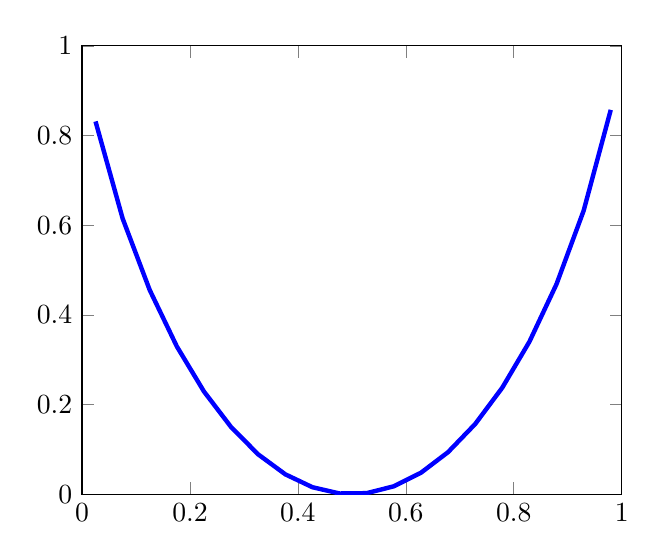
\begin{tikzpicture}
\begin{axis}[ymin=0, ymax=1, xmin=0, xmax=1]
\addplot[samples=200, blue, ultra thick] (x, {1+x*log2(x) + (1-x)*log2(1-x)});
\end{axis}
\end{tikzpicture}
\caption{Capacity as a function of $p$ for a binary symmetric channel}
\end{figure}
At $p=0,1$ the channel transmits perfectly, whilst at $p=\frac{1}{2}$ no information can be transmitted. We can choose to calculate $H(Y)-H(Y|X)$ or $H(X)-H(X|Y)$ to find the information - often one is easier than the other, for example with the binary erasure channel with erasure probability $p$.

$\P(X=0) = \alpha, \P(X=1) = 1-\alpha, \P(Y = 0) = \alpha(1-p), \P(Y=\ast) = p, \P(Y=1) =(1-\alpha)(1-p)$

Then $H(X|Y=0) = 0; H(X|Y = \ast) = H(\alpha); H(X|Y = 1) = 0$, and so $H(X|Y) = pH(\alpha)$. So $C = \max_\alpha (H(\alpha) - pH(\alpha)) = 1-p$, where the maximum value is attained for $\alpha =\frac12$.
\begin{figure}[H]
\centering
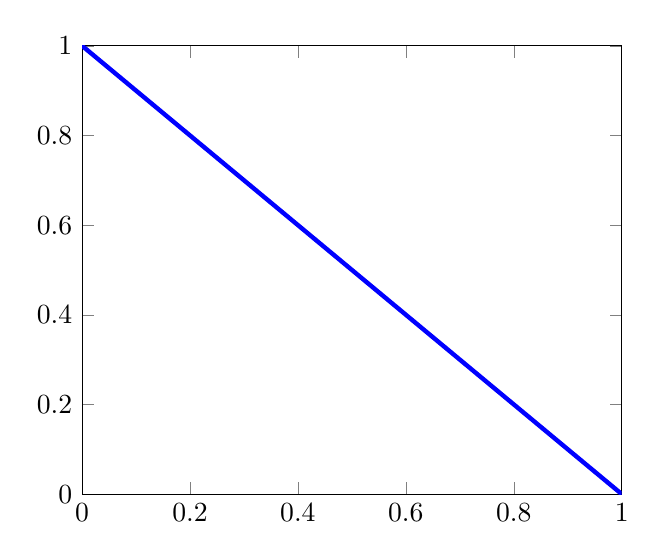
\begin{tikzpicture}
\begin{axis}[ymin=0, ymax=1, xmin=0, xmax=1]
\addplot[samples=200, blue, ultra thick] (x, {1-x});
\end{axis}
\end{tikzpicture}
\caption{Capacity as a function of $p$ for a binary erasure channel}
\end{figure}

We can now model using a channel $n$ times, called the \emph{n\th extension}, i.e. replace input and output alphabets $\mathscr{A}, \mathscr{B}$ by $\mathscr{A}^n, \mathscr{B}^n$.

\begin{lemma}
The $n\th$ extension of a discrete memoryless channel with information capacity $C$ has information capacity $nC$.
\end{lemma}
\begin{proof}
The input $X_1, \ldots, X_n$ determines the output $Y_1, \ldots, Y_n$, and since the channel is memoryless, $H(Y_1,\ldots,Y_n|X_1,\ldots,X_n) = \sum_i H(Y_i|X_1, \ldots, X_n) = \sum_i H(Y_i|X_i)$.
\begin{align*}
I(X_1, \ldots, X_n; Y_1, \ldots, Y_n) &= H(Y_1, \ldots, Y_n) - H(Y_1, \ldots, Y_n|X_1, \ldots, X_n)\\
&= H(Y_1, \ldots, Y_n) - \sum_{i=1}^n H(Y_i|X_i)\\
&\leq \sum_{i=1}^n \left[ H(Y_i) - H(Y_i|X_i)\right]\\
&= \sum_{i=1}^n I(X_i; Y_i) \leq nC
\end{align*}
To finish, we must find $X_1, \ldots X_n$ giving equality - take $X_i$ to be i.i.d. with $I(X_i, Y_i) = C$, giving equality at the second $\leq$. Then the $Y_i$ are i.i.d. so we have equality at the first $\leq$. So the maximum possible value is $nC$.
\end{proof}

\begin{proposition}
For a DMC the operational capacity is at most the information capacity.
\end{proposition}
\begin{proof}
Let $C$ be the information capacity. Suppose that reliable transmission is possible at some $R>C$, i.e. there is a sequence $C_1, C_2, \ldots$, with $C_n$ of length $n$ such that $\lim_{n\to \infty} \rho(C_n) = R$, and $\lim_{n\to\infty} \hat{e}(C_n) = 0$.

We define the \emph{average error rate} $e(C_n) = \frac{1}{|C_n|}\sum_{c \in C_n}\P(\text{error}|c\text{ sent})$, so that $e(C_n) \leq \hat{e}(C_n)$. Hence $e(C_n) \to 0$ as $n \to \infty$. Then let $X$ be a random variable equidistributed in $C_n$. Transmit $X$ and decode to obtain $Y$. So $e(C_n) = \P(X\neq Y)$. Then $H(X) = \log|C_n| = \log\floor{2^{nR}} \geq nR -1$ for sufficiently large $n$. By Fano's inequality,
\begin{align*}
H(X|Y) \leq 1 +e(C_n)\log(|C_n|-1) \leq 1 + e(C_n)n\rho(C_n)
\end{align*}
By the previous proposition,
\begin{align*}
nC \geq I(X,Y) &= H(X) - H(X|Y) \\
&\geq \log|C_n| - (1+e(C_n)n\rho(C_n))\\
&= n\rho(C_n) - e(C_n)n\rho(C_n) - 1\\
\therefore e(C_n)n\rho(C_n) &\geq n(\rho(C_n) - C)-1\\
e(C_n) &\geq \frac{\rho(C_n) - C}{\rho(C_n)} - \frac{1}{n\rho(C_n)} \to \frac{R-C}{R}
\end{align*}
But $R>C$, so $e(C_n) \not\to 0$ as $n \to \infty$. \contr
\end{proof}

\begin{proposition}
Consider the Binary Symmetric Channel with error probability $p$. Let $R < 1- H(p)$. Then there exists a sequence of codes $C_1, C_2, \ldots$, with $C_n$ of length $n$ and size $\floor{2^{nR}}$, such that:
\begin{align*}
\lim_{n \to \infty} \rho(C_n) &= R\\
\lim_{n \to \infty} e(C_n) &= 0
\end{align*}
Note this is $e(C_n)$, not $\hat{e}(C_n)$.
\end{proposition}
\begin{proof}
We use the method of random codes.

Without loss of generality, assume $p <\frac12$. Let $\epsilon > 0$ be such that $p + \epsilon < \frac12$ and $R < 1 - H(p + \epsilon)$. This is always possible since $H$ is continuous. Let $m = \floor{2^{nR}}$ and pick $C \in \mathscr{C} = \{[n,m]-$binary codes$\}$ and random. Note $|\mathscr{C}| = \binom{2^n}{m}$. Let $\mathscr{X}$ be a random variable equidistributed throughout $\mathscr{C}$, say $\mathscr{X} = \{X_1, \ldots, X_m\}$ where the $X_i$ are random variables taking values in $\F_2^n$, such that:
\begin{align*}
\P(X_i = x_i | \mathscr{X} = C) = \begin{cases} \frac1m & x_i \in C \\ 0 & \ow \end{cases}
\end{align*}
Notice that $\P(X_2 = x_2| X_1 = x_1) = \begin{cases} \frac{1}{2^n-1} & x_1\neq x_2\\ 0 & \ow \end{cases}$

Send $X = X_1$ through the BSC, receive $Y$, and decode to obtain $Z$. Under the minimum distance decoding, $\P(X \neq Z) = \frac{1}{|\mathscr{C}|}\sum_{C \in \mathscr{C}} e(C)$.

It then suffices to show that $\P(X \neq Z) \to 0$ as $n \to \infty$. Let $r = \floor{n(p+2)}$.
\begin{align*}
\P(X \neq Z) &\leq \P(B(Y,r) \cap \mathscr{X} \neq \{X\})\\
&= \underbrace{\P(X \notin B(Y,r))}_{(i)} + \underbrace{\P(B(Y,r) \cap \mathscr{X} \supsetneq \{X\})}_{(ii)}
\end{align*}
\begin{itemize}
\item[$(i)$:] $\P(X \notin B(Y,r)) = \P($BSC makes more than $r$ errors$) \to 0$ as $n \to \infty$ by \textbf{9.3}.
\item[$(ii)$:] \begin{align*}
\P(B(Y,r) \cap \mathscr{X} \supsetneq \{X\}) &\leq \sum_{i=2}^m \P(X_i \in B(Y,r)\text{ and }X_1 \in B(Y,r))\\
&\leq \sum_{i=2}^m \P(X_i \in B(Y,r) | X_1 \in B(Y,r))\\
&= (m-1)\frac{V(n,r)-1}{2^n-1}\\
&\leq m\frac{V(n,r)}{2^n}\\
&\leq 2^{nR}2^{nH(p+\epsilon)}2^{-n} = 2^{n(R-(1-H(p+\epsilon)))} \to 0
\end{align*}
since $R < 1-H(p+\epsilon)$
\end{itemize}
\end{proof}
\begin{proposition}
We can replace $e$ by $\hat{e}$ in the previous proposition.
\end{proposition}
\begin{proposition}
Pick $R'$ such that $R<R'<1-H(p)$. Then the previous proposition constructs $C_1', C_2', \ldots$, with $C_n'$ of length $n$, size $\floor{2^{nR'}}$, and $e(C_n') \to 0$ as $n \to \infty$.

Order then codewords of $C_n'$ by $\P($error$|c\sent)$, and delete the worse half them to give $C_n$. Then we have $|C_n| = \floor{\frac{|C_n'|-1}{2}}, \hat{e}(C_n) \leq 2e(C_n')$. Then $\rho(C_n) \to R$ and $\hat{e}(C_n) \to 0$ as $n \to \infty$.
\end{proposition}
Note that:
\begin{enumerate}
\item \textbf{9.12} says we can transmit reliably at any rate $R < 1-H(p)$ so the capacity is at least $1-H(p)$. But, by \textbf{9.10}, the capacity at most $1-H(p)$, and hence the BSC with error probability has capacity $1-H(p)$.

\item The proof shows that good codes exist, but it does not tell us how to find them.
\end{enumerate}
\section{Interlude: An Application to Gambling}
Let $0 < p < 1$, $n>0$, and $0 \leq w <1$. A coin is tossed $n$ times in succession. $P(H) = p$ and, if I pay $k$ ahead of a particular throw, then I get back $kn$ if the throw is head, but nothing if the throw is a tail.

What is my strategy?
\begin{itemize}
\item If $pn <1$, then don't bet - your expected winnings is $<0$.
\item If $pn >1$, then we want to bet, but how much? A larger bet means more winnings, but also more risk. What proportion $w$ of our total wealth should we bet?
\end{itemize}

Note that $w$ is always the same, only the size of the fortune changes. Let the fortune by $X_j$ after the $j\th$ throw. I bet $wX_j$, retaining $(1-w)X_j$. My fortune $X_{j+1}$ after the $(j+1)\th$ throw is:
\begin{align*}
X_{j+1} = \begin{cases} X_j(Xn + 1-w) & j\th \text{ throw is H}\\X_j(1-w) & j\th\text{ throw is T}\end{cases}
\end{align*}
Put $Y_{j+1} = \frac{X_{j+1}}{X_j} = \begin{cases} wn + (1-2) & H \\ 1-w & T\end{cases}$.

Then we try to maximise the log of our fortune: let $\E\log Y_i = \bar{\mu}4, \Var(\log Y_i) = \bar{\sigma}^2$. If $a > 0$ then:
\begin{align*}
\P\left(\left| \frac{\log Y_1+\ldots + \log Y_n}{n} - \bar{\mu}\right|\geq a\right) & \leq \frac{\bar{\sigma}^2}{na^2}
\end{align*}
by Chebyshev's inequality. But $\sum \log Y_i = \log X_i$, so we have:
\begin{align*}
\P\left(\left| \frac{\log X_n}{n} - \bar{\mu}\right|\geq a\right) & \leq \frac{\bar{\sigma}^2}{na^2}
\end{align*}
i.e., for all $\epsilon > 0$, $\delta > 0$, there is some $N$ such that
\begin{align*}
\P\left(\left| n^{-1}\log(X_n) - \bar{\mu}\right| \geq \delta\right) \leq \epsilon\;\;\forall\;\N
\end{align*}
\begin{lemma}
Consider one single toss of a coin with $\P(H) = p < 1$. Suppose that a bet on heads has payout ratio of $n$. Suppose that we have a bankroll of $1$ unit and we bet $w$ on $H$, retaining $1-w$ for $0\leq 1 \leq 1$. If $Y$ is the expected value of our fortune after the throw then
\begin{align*}
\E(\log Y) = p\log(1+(n-1)w) + (1-p)\log(1-w)
\end{align*}
The value of $\E(\log Y)$ is maximised by taking $w = 0$ if $np \leq 1$ and setting $w = \frac{np-1}{n-1}$ if $np > 1$.
\end{lemma}
A better who maximises the $\log$ of his or her fortune is called a \emph{Kelly better}, and is following \emph{Kelly's rule}, since Kelly in 1956 showed how to do this using information theory.

Shannon's Second Coding theorem says that information can be transmitted over a channel at a rate close to the capacity with negligible error rate, provided that we're allowed arbitrarily long messages. Kelly's rule says that a gambler can, with high probability, increase her fortune at a certain optimum rate, provided that she can continue to bet for long enough.

\section{Algebraic Coding Theory}
\subsection{Linear Codes}
A code $C \in \F_2^n$ is \emph{linear} if $0 \in C$ and $x, y \in C \implies x+y \in C$. I.e., $C$ is an $\F_2$-vector subspace of $\F_2^n$. The \emph{rank} of $C$ is its dimension as an $\F_2$-vector subspace. A linear code of length $n$, rank $k$ is denoted an \emph{(n,k)-code}, using round brackets instead of square brackets. If its minimum distance is $d$, it is an $(n,k,d)$-code.

Let $v_1, \ldots, v_k$ be a basis for $C$. Then $C = \left\{\sum_{i=1}^k \lambda_i v_i : \lambda_i \in \F_2\right\}$, so $|C| = 2^k$, and $(n,k)$-codes are $[n,2^k]$-codes. The information rate is then $\frac{k}{n}$.

The \emph{weight} of $x \in \F_2^n$, denoted $w(x) = d(x,0)$.

\begin{lemma}
The minimum distance of a linear code is the minimum weight of a non-zero codeword.
\end{lemma}
\begin{proof}
Suppose $d(x,y) = d$. Then $d(x+y, y+y) = d(x+y,0) = w(x+y) = d$, and $x+y \in C$ as $C$ is linear.
\end{proof}

For $x, y \in \F_2^n$, let $x\cdot y = \sum_{i=1}^n x_iy_i \in \F_2$. Note that there are $x \neq 0$ with $x\cdot x = 0$. We then define the \emph{parity check code} defined by $P \subseteq \F_2^n$ to be $C = \{x \in \F_2^n : p\cdot x = 0 \;\forall p\in P\}$.

We've already seen some examples of this:
\begin{itemize}
\item $P = \{111\ldots 1\}$ gives the simple parity check code.
\item $P = \{1010101,0110011,0001111\}$ gives Hamming's original code.
\end{itemize}
\begin{lemma}
Every parity check code is linear.
\end{lemma}
\begin{proof}
$0 \in C$ as $p\cdot 0 = 0\;\forall p \in P$. If $x, y \in C$, then $p\cdot(x+y)=p\cdot x+p\cdot y = 0+0 = 0$, so $x+y \in P$,
\end{proof}

If $C \subset \F_2^n$ is a linear code, then the \emph{dual code} of $C$, $C^{\bot} = \{x\in\F_2^n: x\cdot y =0 \;\forall y \in C\}$.

This is a parity check code so is linear. Note that $C \cap C^{\bot}$ can be larger than $\{0\}$.

\begin{lemma}
$\rank(C) + \rank(C^{\bot}) = n$
\end{lemma}
\begin{proof}
Linear algebra using $C^{\bot}$ is the annihilator of $C$, or see later.
\end{proof}
\begin{lemma}
If $C$ is linear, then $(C^{\bot})^{\bot} = C$, and in particular $C$ is a parity check code.
\end{lemma}
\begin{proof}
If $x \in C$ then $x \cdot y = 0$ for all $y \in C^{\bot}$. Hence $x \in (C^{\bot})^{\bot}$, and so $C \subseteq (C^{\bot})^{\bot}$.

Then $\rank(C) = n - \rank(C^{\bot}) = n-(n-\rank((C^{\bot})^{\bot})) = \rank(C^{\bot})^{\bot})$, and so $C = (C^{\bot})^\bot$.
\end{proof}

Let $C$ be a $(n,k)$-code. Then we have a couple of useful matrices:
\begin{enumerate}
\item A \emph{generator matrix} $G$ for $C$ is a $k\times n$ matrix with rows a basis of $C$.
\item A \emph{parity check matrix} $H$ for $C$ is a generator matrix for $C^\bot$.
\end{enumerate}
The codewords in $C$ can be viewed as linear combinations of row of $G$, or as linear dependence relations between the columns of $H$.

\subsection{Syndrome Decoding}
If $C$ is an $(n,k)$linear code, then the syndrome of $x \in \F^n_2$ is $Hx$. If we receive $x = c+z$ where $c$ is a codeword and $z$ is an error pattern, then $Hx = Hc+Hz = Hz$.

If $C$ is $e$-error correcting, we pre-compute $Hz$ for all $z$ with $w(z) \leq e$. On receiving $x \in \F_2^n$ we look for $Hx$ in our list. Then if $Hx = Hz$, $H(x-z) = 0$, so $c = x-z \in C$ with $d(x,c) \leq e$.

Codes $C_1, C_2 \in \F_2^n$ are \emph{equivalent} if, reordering each codeword of $C_1$ using the same permutation each time, gives the codewords of $C_2$. Usually we only consider codes up to equivalence.

\begin{proposition}
Every $(n,k)$-linear code is equivalent to one with generator matrix of the form $G = (I_k | B)$ for some $k \times (n-k)$ matrix $B$.
\end{proposition}
\begin{proof}
Using elementary row operations we can transform $G$ into row echelon form
\begin{align*}
G_{ij} = \begin{cases} 0 & j < \ell(i)\\1 & j = \ell(i) \end{cases}
\end{align*}
for some $\ell(1) <\ell(2) < \ldots < \ell(k)$. Permuting the columns replaces the code by an equivalent code, and so \textsc{wlog} we can assume $\ell(i) = i$ for all $i$. Then we can cancel all the non-zero off diagonal entries on the left hand square of $G$, to get it in the form $(I_k|B)$.
\end{proof}
If we have a message $y \in \F_2^k$ viewed as a row matrix, we encode it as $yG$. If $G$ is in the form of \textbf{11.5}, then $yG = (y|yB)$ where $y$ is the message and $yB$ are check digits. Any code whose codewords can be split up in this manner is called \emph{systematic}. This form of the generator matrix will let us prove \textbf{11.3} without working with dual spaces:
\begin{proof}[Proof of 11.3]
Without any loss of generality, we may take $C$ to have generator matrix $G = (I_k|B)$. $G$ has $k$ linearly independent columns, so the linear map $c:\F_2^n \to \F_2^k; x \mapsto Gx$ is surjective with kernel $C^{\bot}$. By the rank nullity, $\dim \F_2^n = \rank C + \rank C^{\bot}$.
\end{proof}
\begin{lemma}
An $(n,k)$-linear code with generator matrix $G = (I_k |B)$ has parity check matrix $H = (B^t |I_{n-k})$.
\end{lemma}
\begin{proof}
$GH^t = (I_k |B)\left(\frac{B}{I_{n-k}}\right) = B+B = 0$, so the rows of $H$ generate a subcode of $C^{\bot}$. But the rank of $H = n-k$since $H$ contains $I_{n-k}$ as a submatrix and $n-k = \rank C^{\bot}$, so $C^{\bot}$ has generator matrix $H$, and $H$ is a parity check matrix for $C$.
\end{proof}
\section{Examples of Codes}
\subsection{Hamming Codes}
For $d \geq 1$ let $n = 2^d - 1$. Let $H$ be the $d \times n$ matrix whose columns are the non zero elements of $\F_2^d$. The \emph{Hamming (n,n-d)-code} is the linear code with parity check matrix $H$. For example with $d = 3$:
\begin{align*}
H = \begin{pmatrix} 1&0&1&0&1&0&1\\0&1&1&0&0&1&1\\0&0&0&1&1&1&1\end{pmatrix}
\end{align*}
\begin{lemma}
The minimum distance of the $(n,n-d)$-Hamming code $C$ is $d(C) = 3$. It is a perfect 1-error correcting code.
\end{lemma}
\begin{proof}
The codewords of $C$ are dependence relations between the columns of $H$. Any two columns of $H$ are linearly independent, so there are no codewords of weight at most 2. Hence $d(C) \geq 3$. Noting that $11100\ldots 0 \in C$, we have $d(C) = 3$. It is 1-error correcting by \textbf{5.3}. Moreover, $\frac{2^n}{V(n,1)} = \frac{2^n}{n+1} = 2^{n-d} = |C|$, so $C$ is perfect.
\end{proof}
\subsection{Reed-Muller Codes}
Take some finite set $X$ of size $n$ say. Then there is a correspondence between $\powset(X)$ and $\F_2^n$ given by indicator functions. Moreover, we have that the following set-theoretic operations in $\powset(X)$ correspond to vector operations on $\F_2^n$:
\begin{align*}
A \Delta B = (A \setminus B) \cup (B \setminus A) &\xleftrightarrow{\hspace{2cm}} x+y = (x_1+y_1,\ldots, x_n+y_n)\\
A \cap B &\xleftrightarrow{\hspace{2cm}} x \wedge y = (x_1y_1, \ldots, x_ny_n)
\end{align*}
Take $X = F_2^d$, so $n = 2^d$. Let $v_0 = \one_X = (1,1,\ldots, 1)$. Let $v_i = \one_{H_i}$ for $1 \leq i \leq d$, where $H_i = \{p \in X : p_i = 0\}$, the coordinate hyperplane.

Then the \emph{Reed-Muller code RM(d,r)} of order $r$ where $0\leq r\leq d$ of length $2^d$ si the linear code spanned by $v_0$ and all wedge products of $r$ or fewer of the $v_i$. By convention, the empty wedge is $v_0$. For example, with $d = 3, X = \F_2^3$ in binary number order:
\begin{center}
\begin{tabular}{c|cccccccc}
$X$&000&001&010&011&100&101&110&111\\\hline
$v_0$&1&1&1&1&1&1&1&1\\
$v_1$&1&1&1&1&0&0&0&0\\
$v_2$&1&1&0&0&1&1&0&0\\
$v_3$&1&0&1&0&1&0&1&0\\
$v_1\wedge v_2$&1&1&0&0&0&0&0&0\\
$v_2\wedge v_3$&1&0&0&0&1&0&0&0\\
$v_1\wedge v_3$&1&0&1&0&0&0&0&0\\
$v_1\wedge v_2\wedge v_3$&1&0&0&0&0&0&0&0
\end{tabular}
\end{center}
Note that:
\begin{itemize}
\item RM(3,0): spanned by $v_0$, is a repetition code of length 8.
\item RM(3,1): spanned by $v_0,v_1,v_2,v_3$, is a parity check extension of Hamming's original code.
\item RM(3,2): an $(8,7)$-code, which is actually a simple parity check code.
\item RM(3,3): the trivial code for $\F_2^8$.
\end{itemize}
\begin{theorem}
\item
\begin{enumerate}
\item The vectors $v_{i_0} \wedge \ldots \wedge v_{i_j}$ form a basis for $\F_2^n$.
\item The rank of $RM(d,r) = \sum_{s=0}^r \binom{d}{s}$.
\end{enumerate}
\end{theorem}
\begin{proof}
\item
\begin{enumerate}
\item We've listed $\sum_{s=0}^d \binom{d}{s} = (1+1)^d = 2^d$ vectors, so it's enough to check spanning, i.e. that $RM(d,d) = \F_2^n$. Let $p \in X$. Put $y_i = \begin{cases} v_i & p_i=0\\ v_0+v_i & p_i=1\end{cases}$. Then $\one_{\{p\}} = y_1 \wedge \ldots \wedge y_d$, and we can expand this using distributivity to get $\one_{\{p\}} \in RM(d,d)$. But $\{\one_{\{p\}} : p \in X\}$ spans $\F_2^n$, and so the given vectors form a basis.
\item $RM(d,r)$ is spanned by $v_{i_1} \wedge \ldots \wedge v_{i_s}$ for $1 \leq i < \ldots <i_s \leq d$ with $0 \leq s \leq r$. These vectors are linearly independent by part \textit{1.}, and so form a basis. Hence $\rank RM(d, r) = \sum_{s=0}^r \binom{d}{s}$.
\end{enumerate}
\end{proof}

Let $C_1, C_2$ be linear codes of length $n$ with $C_2 \subseteq C_1$. The \emph{bar product} $C_1|C_2 = \{(x|x+y) : x \in C_1, y \in C_2\}$. It is a linear code of length $2n$.
\begin{lemma}
\item
\begin{enumerate}
\item $\rank(C_1|C_2) = \rank C_1 + \rank C_2$
\item $d(C_1|C_2) = \min\{2d(C_1), d(C_2)\}$
\end{enumerate}
\end{lemma}
\begin{proof}
\item
\begin{enumerate}
\item $C_1$ has a basis $x_1, \ldots, x_k$, $C_2$ has a basis $y_1, \ldots, y_\ell$. Then $C_1|C_2$ has a basis given by $\{(x_i|x_i: 1\leq i \leq k\}\cup\{(0|y_i):1\leq i \leq \ell\}$.

So $\rank(C_1|C_2) = k + \ell = \rank C_1 + \rank C_2$.

\item Take $x \in C_1, y \in C_2$ not both zero so that $(x|x+y) \in C_1|C_2$ is non-zero. Then if $y \neq 0, w(x|x+y) \geq w(y) \geq d(C_2)$. Meanwhile if $y=0$, then $w(x|x+y) = 2w(x) \geq 2d(C_1)$.

Hence $d(C_1|C_2) \geq \min \{2d(C_1), d(C_2)\}$. For equality, take $x$ of weight $d(C_1)$, $y$ of weight $d(C_2)$. Then $x|0$ or $0|y$ attains the bound.
\end{enumerate}
\end{proof}
\begin{theorem}
\item
\begin{enumerate}
\item $RM(d,r) = RM(d-1,r-1)|RM(d-1,r-1)$
\item $RM(d,r)$ has minimum distance $2^{d-r}$
\end{enumerate}
\end{theorem}
\begin{proof}
\item
\begin{enumerate}
\item $RM(d-1, r-1) \subseteq RM(d-1, r)$, so the bar product is defined. Order the elements of $X = \F_2^d$ such that $v_d = (0\ldots 0 |1\ldots 1)$ where each part has length $2^{d-1}$, and let $v_i = (v_i'|v_i')$

Take $z \in RM(d,r)$, then $z$ is a sum of wedge products of $v_1, \ldots, v_d$. So $z = x+(y \wedge v_d)$ for $x,y$ sums of wedge products of $v_1, \ldots, v_{d-1}$. Then $x = (x'|x')$ for some $x' \in RM(d-1,r)$, and $y = (y'|y')$ for some $y' \in RM(d-r, r-1)$.

Then $z = (x'|x') + (y'|y')\wedge (0\ldots 0|1\ldots 1) = (x'|x'+y') \in RM(d-1,r)|RM(d-1,r-1)$. The converse is similar, or argue using cardinalities.

\item If $r=0$ then $RM(d,0)$ is a repetition code of length $n = 2^d$, which has minimum distance $2^{d-0}$. If $r=d$, then $RM(d,d)$ is the trivial code which has minimum distance $1=2^{d-d}$. We prove the case $0 < r < d$ by induction on $d$. The minimum distance of $RM(d-1,r) = 2^{d-1-r}$ and of $RM(d-1,r-1)$ is $2^{d-r}$. So by the previous lemma, the minimum distance of $RM(d,r) = \min \{2\cdot 2^{d-r-1}, 2^{d-r}\} = 2^{d-r}$.
\end{enumerate}
\end{proof}

\section{Cyclic Codes}
A linear code $C \subseteq \F_2^n$ is \emph{cyclic} if $(a_0, a_1, \ldots, a_{n-1}) \in C \implies (a_{n-1}, a_0, a_1, \ldots, a_{n-2}) \in C$, i.e. rotations of all of our codewords are also codewords. We can identify $\F_2^n$ with $\F_2[x]/(x^n-1)$, via $(a_0,a_1, \ldots, a_{n-1}) \leftrightarrow a_0 + a_1x+\ldots+a_{n-1}x^{n-1}$.
\begin{lemma}
$C \subseteq \F_2[x]/(x^n-1)$ is cyclic if and only if $C \trianglelefteq \F_2[x]/(x^n-1)$.
\end{lemma}
\begin{proof}
If $g(x) = a_0 + a_1 x + \ldots + a_{n-1} x^{n-1} \mod x^n-1$ then $xg(x) = a_{n-1}+a_0 x + \ldots x_{n-2}x^{n-2}$, and so if $C \subseteq \F_2[x]/(x^n-1)$ is closed under multiplication by $x$ then $C$ has this cyclic property.

But we also know $C$ is linear, and so this gives us closure under addition of codewords, so by repeated application of additions and multiplications, we have $f(x)g(x) \in C$ for any polynomial $f(x)$, and in particular $C$ is an ideal of $\F_2[x]/(x^n-1)$.
\end{proof}

\begin{theorem}
Let $C \subset \F_2[x]/(x^n-1)$ be a cyclic code. Then there is a unique $g(x) \in \F_2[x]$ such that:
\begin{enumerate}
\item $C = \{f(x)g(x) \mod x^n-1 : f(x) \in \F_2[x]\}$
\item $g(x) | x^n-1$
\end{enumerate}
In particular, $p(x) \in \F_2[x]$ represents a codeword if and only $g(x)|p(x)$. We say $g(x)$ is \emph{the generator polynomial} of $C$.
\end{theorem}
\begin{proof}
Let $g(x) \in \F_2[x]$ be of least degree representing a non-zero codeword. Then $\deg g < n$. Since $C$ is cyclic, we have $\supseteq$ in \textit{1.}

Let $p(x) \in \F_2[x]$ represent a codeword. Then $p(x) = q(x)g(x)-r(x)$ where $\deg r < \deg g$. So $r(x) = p(x) - q(x)g(x) \in C$ as $C$ is an idea and so by minimality of $\deg g$, $r(x) = 0$. So $g(x)|p(x)$.

For uniqueness, suppose $g_1(x), g_2(x)$ both satisfy the properties. Then $g_1(x)|g_2(x)$ and $g_2(x)|g_1(x)$, so $g_1(x) = g_2(x)$.
\end{proof}
We can actually think of $C$ as a vector space over $\F_2$:
\begin{lemma}
Let $C$ be a cyclic code of length $n$ generated by $g(x) = a_0 + a_1 x+\ldots +a_{k}x^k$, $a_k \neq 0$. Then $C$ has $g(x), xg(x), \ldots, x^{n-k-1}g(x)$, and in particular $\rank C = n-k$.
\end{lemma}
\begin{proof}
Suppose $f(x)g(x) = 0 \mod x^n-1$ for some $f(x) \in \F_2[x]$ with $\deg f < n-k$. Then $\deg fg < n$, so $f(x)g(x) = 0 \implies f(x) = 0$, and so these terms are linearly independent.

For spanning, let $p(x)$ represent a codeword. Since $g(x)$ is the generator polynomial, $g(x)|p(x)$, i.e. $p(x) = f(x)g(x)$ for some $f(x)$. But $\deg f = \deg p - \deg g < n-k$, so $p(x)$ is in the span of $g(x), xg(x), \ldots, x^{n-k-1}g(x)$.
\end{proof}
\begin{corollary}
The $(n-k)\times n$ generator matrix is:
\begin{align*}
G = \begin{pmatrix} a_0 & a_1 & a_2 & \cdots & a_k & 0 & \cdots & 0 \\
0 & a_0 & a_1 & \cdots & a_{k-1} & a_k & \cdots & 0\\
\vdots & & \ddots & \ddots & & \ddots & \ddots & \vdots\\
0 & 0 & 0 & \cdots & a_0 & a_1 & \cdots & a_k\end{pmatrix}
\end{align*}
\end{corollary}
\begin{lemma}
The \emph{parity check polynomial} $h(x) \in \F_2[x]$ is defined by $x^n-1 = g(x)h(x)$. If $h(x) = b_0 + b_1x + \ldots + b_{n-k}x^{n-k}$, then the parity check matrix is the $k \times n$ matrix:
\begin{align*}
H = \begin{pmatrix} b_{n-k} & b_{n-k-1} & \cdots & b_1 & b_0 & 0 & \cdots & 0 \\
0 & b_{n-k} & \cdots & b_2 & b_1 & b_0 & \cdots & 0 \\
\vdots & & \ddots & & \ddots  & \ddots & \ddots & \vdots \\
0 & 0 & \cdots & b_{n-k} & \cdots & \cdots & b_1 & b_0
\end{pmatrix}
\end{align*}
\end{lemma}
\begin{proof}
Indeed the dot product of the $i\th$ row of $G$ and the $j\th$ column of $H$ is the coefficient of $x^{n-k-i+j}$ in $g(x)h(x)$. The coefficients of $g(x)h(x) = x^n-1$ are 0, and hence the rows of $G$ and $H$ are orthogonal. Also, $\rank H = k = rkC^{\bot}$, so $H$ is a parity check matrix.
\end{proof}
Note that the check polynomial is the reverse of the generator polynomial for the dual code.
\begin{lemma}
If $n$ is odd then $x^n-1 = f_1(x) \ldots f_t(x)$ with $f_i(x)$ distinct irreducibles in $\F_2[x]$. In particular, there are $2^t$ cyclic codes of length $n$.
\end{lemma}
\begin{proof}[Proof*]
If $x^n-1$ has a repeated factor then there is a field extension $K/\F_2$ such that $x^n-1 = (x-\lambda)^2 g(x)$ for some $\lambda \in K, g(x) = \F_2[x]$. Taking formal derivatives, $nx^{n-1} = 2(x-\lambda)g(x) + (x-\lambda)^2 g'(x)$.

So $n\lambda^{n-1} = 0 \implies \lambda = 0$, and so $0 = \lambda^n = 1$ \contr.
\end{proof}

\section{BCH Codes}
Let $n$ be an odd integer, and $r \geq 1$ such that $2^r \equiv 1 \mod n$, which exists since $(2,n) = 1$. Letting $K = \F_{2^r}$, let $\mu_n(K) = \{x\in K:x^n = 1\}\leq K^{\ast}$. Since $n|(2^r-1) = |K^{\ast}|$, $\mu_n(K)$ is a cyclic group of order $n$. So $\mu_n(K) = \{1, \alpha, \ldots, \alpha^{n-1}\}$ for some $\alpha \in K$ called a primitive $n\th$ root of unity.

The cyclic code of length $n$ with \emph{defining set} $A \subseteq \mu_n(K)$ is:
\begin{align*}
C = \{f(x) \mod x^n-1 : f(x) \in \F_2[x], f(a) = 0 \forall a \in A\}
\end{align*}
The \emph{generator polynomial} is the nonzero polynomial $g(x)$ of least degree with $g(x) = 0$ for all $a \in A$. Equivalently, $g(x)$ is the lowest common multiple of the minimal polynomials of the elements $a \in A$.

The cyclic code with defining set $\{\alpha, \alpha^2, \ldots, \alpha^{\delta - 1}\}$ is called a \emph{BCH Code} with \emph{design distance} $\delta$.

\begin{lemma}[Vandermonde Determinant]
\begin{align*}
\left| \begin{pmatrix}
1 & 1 & \cdots & 1\\
x_1 & x_2 &  \cdots & x_n \\
x_1^2 & x_2^2 & \cdots & x_n^2 \\
\vdots & \vdots & &\vdots \\
x_1{^n-1} & x_2^{n-1} & \cdots x_n^{n-1}
\end{pmatrix}\right|
= \prod_{1\leq j<i\leq n} (x_i - x_j)
\end{align*}
\end{lemma}
\begin{proof}
Exercise.
\end{proof}
\begin{theorem}
A BCH code $C$ with design distance $\delta$ has $d(C) \geq \delta$.
\end{theorem}
\begin{proof}
Consider:
\begin{align*}
H = \begin{pmatrix}
1 & \alpha & \alpha^2 & \cdots & \alpha^{n-1}\\
1 & \alpha^2 & \alpha^4 & \cdots & \alpha^{2(n-1)}\\
\vdots & \vdots & \vdots & &\vdots \\
1 & \alpha^{\delta-1} & \alpha^{2(\delta-1)} & \cdots & \alpha^{(\delta-1)(n-1)}
\end{pmatrix}
\end{align*}
By the Vandermonde determinant the columns of $H$ are linearly independent. But any codeword of $C$ is a dependence relation between columns of $H$. Hence every non-zero codeword has weight $\geq \delta$. Hence $d(C) \geq \delta$.
\end{proof}
Note that $H$ is not a parity check matrix as defined, because the entries are in $K$ and not in $\F_2$.

\subsection{Decoding BCH Codes}
Let $C$ be a cyclic code with defining set $\{\alpha, \alpha^2, \ldots, \alpha^{\delta-1}\}$, where $\alpha \in K$ is a primitive $n\th$ root of unity. Then we should be able correct $\floor{\frac{\delta-1}{2}} = t$ errors. We send $c\in C$ and receive $r = c+e$ where $e$ is an error pattern with $\leq t$ non-zero entries. Now we have a correspondence $\F_2^n \leftrightarrow \F_2[x]/(x^n-1)$, so $r, c, e \leftrightarrow r(x), c(x), e(x)$. 

Then we define the \emph{error locator polynomial} to be $\sigma(x) = \prod_{i \in \mathcal{E}} (1-\alpha^i X) \in K[x]$, where $\mathcal{E} = \{0 \leq i\leq n-1:e_i = 1\}$.

\begin{theorem}
Assume $\deg \sigma = |\mathcal{E}| \leq t$. Then $\sigma(x)$ is the unique polynomial in $K[x]$ of least degree such that:
\begin{itemize}
\item $\sigma(0) = 1$
\item $\sigma(x) \sum_{j=1}^{2t} r(\alpha^i)x^j = \omega(x)$
\end{itemize}
for some $\omega(x) \in K[x]$ with $\deg \omega \leq t$.
\end{theorem}
\begin{proof}
Define $\omega(x) = -x\sigma'(x)$. Then:
\begin{align*}
\omega(x) = \sum_{i\in \mathcal{E}}\alpha^i x\prod_{i \neq j \in \mathcal{E}}(1-\alpha^j x)
\end{align*}
Working in $K[[x]]$, the ring of formal power series, we get:
\begin{align*}
\frac{\omega(x)}{\sigma(x)} &= \sum_{i \in \mathcal{E}}\frac{\alpha^i x}{1-\alpha^i x} \\
&= \sum_{i \in \mathcal{E}}\sum_{j=1}^\infty (\alpha^i x)^j\\
&= \sum_{j=1}^\infty x^j \sum_{i \in \mathcal{E}} (\alpha^j)^i\\
&= \sum_{j=1}^\infty e(\alpha^j) x^j
\end{align*}
So $\omega(x) = \sigma(x)\sum_{j\geq 1} e(\alpha^j)x^j$. By the definition of $C$, $c(\alpha^i) = 0$, and so $r(\alpha^i) = e(\alpha^i)$. Hence:
\begin{align*}
\sigma(x)\sum_{j=1}^{2t} r(\alpha^j)x^j = \omega(x) \mod x^{2t+1}
\end{align*}
This verifies \textit{1.} and \textit{2.} with $\omega(x) = -x\sigma'(x)$, so $\deg \omega =\deg \sigma =|\mathcal{E}| \leq t$. 

For uniqueness, suppose we have $\tilde{\sigma}, \tilde{\omega}$ also satisfying these properties with $\deg \tilde{\sigma} \leq \deg\sigma$. Then if $i \in \mathcal{E}$, $\omega(\alpha^{-i}) = \prod_{i\neq j\in\mathcal{E}} (1-\alpha^{j-i}) \neq 0$ and $\sigma(x), \omega(x)$ are coprime.

Then $\sigma(x)\tilde{\omega}(x) \equiv \tilde{\sigma}(x)\omega(x) \mod x^{2t-1}$, so $\sigma(x)\tilde{\omega}(x) = \tilde{\sigma}(x)\omega(x)$. But $\sigma(x), \omega(x)$ are coprime, so $\sigma(x)|\tilde{\sigma}(x)$. By assumption, $\deg\tilde{\sigma}(x) \leq \deg \sigma$, so $\tilde{\sigma} = \lambda \sigma$ for some $\lambda \in K$. But $\lambda \sigma(0) = \lambda = 1$, so $\sigma = \tilde{\sigma}$.
\end{proof}

So to decode a BCH code we have the following procedure:
\begin{itemize}
\item We receive $r(x)$.
\item Compute $\sum_{j=1}^{2t} r(\alpha^{j})x^j$.
\item Set $\sigma(x) = 1+ \sigma_1x+\ldots + \sigma_t x^t$ and compare coefficients of $x^i$ for $t+1\leq i\ 2T$ to obtain linear equations for $\sigma_1, \ldots, \sigma_t$.
\item Solve these via Gaussian elimination taking solutions of least degree.
\item Compute $\mathcal{E} = \{i: \sigma(\alpha^{-i}) = 0\}$, and check that $|\mathcal{E}| = \deg \sigma$.
\item Set $e(x) = \sum_{i \in \mathcal{E}} x^i$, $c(x) = r(x)+e(X)$, and check $c(x)$ is a codeword.
\end{itemize}

\section{Shift Registers}
A \emph{general feedback shift register} is a function $f:\F_2^d \to \F_2^d$ of the form $f(x_0, \ldots, x_{d-1}) = (x_1, \ldots, x_{d-1}, C(x_0, \ldots, x_{d-1}))$ for some function $C:\F_2^d \to \F_2^d$. We say the register has \emph{length} $d$.
\begin{figure}[H]
\begin{center}
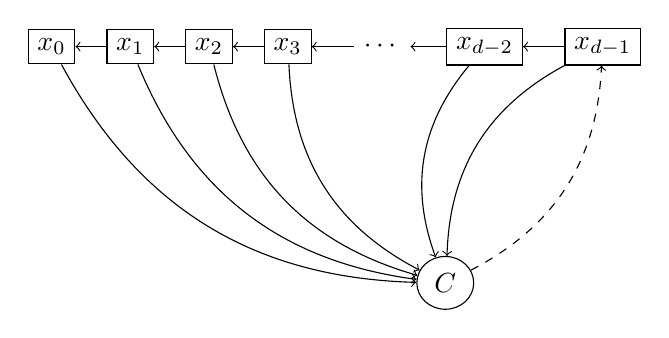
\begin{tikzpicture}
\node[rectangle, draw] (0) at (-5,3) {$x_0$};
\node[rectangle, draw] (1) at (-4,3) {$x_1$};
\node[rectangle, draw] (2) at (-3,3) {$x_2$};
\node[rectangle, draw] (3) at (-2,3) {$x_3$};
\node[rectangle, draw] (4) at (.5,3) {$x_{d-2}$};
\node[rectangle, draw] (5) at (2,3) {$x_{d-1}$};
\node (6) at (-0.8,3) {$\cdots$};
\node[ellipse, draw] (C) at (0,0) {$C$};
\draw[->] (1)--(0);
\draw[->] (2)--(1);
\draw[->] (3)--(2);
\draw[->] (6)--(3);
\draw[->] (4)--(6);
\draw[->] (5)--(4);
\draw[->] (0) edge[bend right] (C);
\draw[->] (1) edge[bend right] (C);
\draw[->] (2) edge[bend right] (C);
\draw[->] (3) edge[bend right] (C);
\draw[->] (4) edge[bend right] (C);
\draw[->] (5) edge[bend right] (C);
\draw[->] (C) edge[bend right, dashed] (5);




\end{tikzpicture}
\end{center}
\end{figure}

A register is \emph{linear} (LFSR) if $C$ is a linear map, say $(x_0, \ldots, x_{d-1}) \mapsto \sum_{i=0}^{d-1} a_ix_i$. The \emph{initial fill} $(y_0, \ldots, y_{d-1})$ produces an output sequence (or stream) $(y_n)_{n\geq 0}$, where $y_{n+d} = C(y_n, y_{n+1}), \ldots, y_{n+d-1})$. 

So in the linear case we have a sequence determined by a recurrence relation with \emph{auxiliary polynomial} $P(x) = x^d + a_{d-1}x^{d-1}+\ldots+a_1 x+a_0$.

The \emph{feedback polynomial} is $\tilde{P}(x) = a_0 x^d+a_1 x^{d-1}+\ldots+a_{d-1}x + 1 = x^{\deg P}P(x^{-1})$.

\begin{lemma}
The sequence $(y_n)_{n\geq 0}$ in $\F_2$ is the output from an LFSR with auxiliary polynomial $P(x)$ if and only if $G(x)\tilde{P}(x) = A(x)$ where $G(x)$ is the polynomial $\sum_{i\geq 0}y_i x^i$, and $A(x)$ is some polynomial of degree $< \deg P$.
\end{lemma}
\begin{proof}
Let $P(x), \tilde{P}(x)$ be as above. The condition holds if and only if the coefficient of $x^n$ in $G(x)\tilde{P}(x)$ is 0 for $n \geq d$, which happens if and only if $\sum_{i=0}^{d}a_iy_{n-d+i} =0$ for $n \geq d$.

This happens iff $y_{n+d} = \sum_{i=0}^{d-1}a_i y_{n-i}$ for $n \geq 0$, i.e. if $(y_n)_{n \geq 0}$ comes from a LFSR with feedback polynomial $\tilde{P}(x)$.
\end{proof}
Compare this proof with the decoding procedure for BCH codes
\subsection{Berlekamp-Massey Algorithm}
This is an algorithm to find the shortest LFSR for a given binary output stream. Let $(x_n)$ be the output of an LSFR. We want to find $d$ and $a_0, a_1, \ldots, a_{d-1} \in \F_2$ such that $x_{n+d} = \sum_{i=0}^{d-1} a_i x_{n+i}$ for all $n \geq 0$.

Translating this into a linear algebra problem, we have:
\begin{align*}
\underbrace{\begin{pmatrix}
x_0 & x_1 & \cdots x_d \\
x_1 & x_2 & \cdots x_{d+1} \\
\vdots & \vdots &&\vdots \\
x_{d} & x_{d+1} & \cdots & x_{2d}
\end{pmatrix}}_{A_d} \begin{pmatrix}
a_0 \\ a_1 \\ \vdots \\ a_{d}
\end{pmatrix} = 0\tag{\ast}
\end{align*}
Then if we know the register has length $\geq r$, start with $d=r$. For each $i$, compute $\det A_i$.
\begin{itemize}
\item If $\det A_i \neq 0$ then $d > i$, so replace $i$ by $i+1$ and repeat.
\item If $\det A_i = 0$, we can solve $(\ast)$ using Gaussian elimination, and test the solution over as many terms of the sequence as we like. If it fails, then $d>i$, and replace $i$ by $i+1$ and continue.
\end{itemize}
We'll return to this in \textsection 17.

\section{Cryptography}
\subsection{Introduction and Examples}
We want to modify a message such that it becomes unintelligible to an eavesdropper. Certain secret information will be shared by $A, B$, called the \emph{key}, which lies in a space $\mathcal{K}$. The unencrypted message will be called \emph{plaintext}, lying in $\mathcal{M}$. The encrypted message will be called \emph{ciphertext}, lying in $\mathcal{C}$. A \emph{cryptosystem} consists of sets ($\mathcal{K, M, C}$), together with functions:
\begin{align*}
e: \mathcal{M}\times\mathcal{K} &\to \mathcal{C}\tag{\text{encrypt}}\\
d: \mathcal{C}\times\mathcal{K} &\to \mathcal{M}\tag{\text{decrypt}}
\end{align*}
with the property that $d(e(m,k),k) = m$ for all $m \in \mathcal{M}, k \in \mathcal{K}$.

\example{s}: $\mathcal{M}=\mathcal{C} = \Sigma=\{A, B, \ldots, Z\}$
\begin{itemize}
\item \underline{Simple substitution:} $\mathcal{K} = \{$permutations of $\Sigma\}$. Then each letter is encrypted as the image under the chosen permutation.
\item \underline{Vigen\`{e}re cipher:} $\mathcal{K} = \Sigma^d$ for some $d \in \N$. We identify $\Sigma$ and $\Z/26\Z$. and write the key repeatedly below the message and add mod 26:
\setul{5pt}{.8pt}
\begin{align*}
&\texttt{ATTACKATDAWN}\\
+\;&\ul{\texttt{LEMONLEMONLE}}\\
=\;&\texttt{LXFOPVEFRNHR}
\end{align*}
If $d=1$ this is called a \emph{Caesar cipher}.
\end{itemize}
\subsection{Breaking the Cryptosystem}
Some attacker $E$ might know:
\begin{itemize}
\item The functions $e$ and $d$ (i.e. the mechanics of the cryptography)
\item The probability distributions  on $\mathcal{M}, \mathcal{K}$.
\end{itemize}
She does not know the key however. Her goal is to recover the plaintext from the ciphertext. There are three possible levels of attack:
\begin{itemize}
\item[Level 1:] Ciphertext only - she just knows some piece of ciphertext.
\item[Level 2:] Known plaintext - she possesses a considerable length of plaintext and matching ciphertext.
\item[Level 3:] Chosen plaintext - she may acquire the ciphertext for any plaintext she wants to.
\end{itemize}
For example, the substitution cipher and Vigen\`ere cipher fail at level 2 for sufficiently random messages. They can in fact fail at level 1, for instance if we know the source is a passage of English text. For modern work, level 3 is desirable.

We model the keys and messages as independent random variables $K, M$ taking values in $\mathcal{K, M}$. Put $C = e(M,K)$. We say a cryptosystem has \emph{perfect secrecy} if $M, C$ are independent, or equivalently if $I(M; C) = 0$.

\begin{lemma}
If a code has perfect secrecy then $|\mathcal{K}|\geq |\mathcal{M}|$.
\end{lemma} 
\begin{proof}
Pick $m_0 \in \mathcal{M}, k_0 \in \mathcal{K}$, both with strictly positive probability. Then $c_0 = e(m_0, k_0)$ also has strictly positive probability. Then for all $m \in \mathcal{M}$:
\begin{align*}
\P(C=c_0) = \P(C=c_0|M=m)
\end{align*}
by perfect secrecy. Hence for any $m \in \mathcal{M}$ there is a $k \in \mathcal{K}$ with $e(m,k) = c_0$. If two messages $m_1, m_2$ encrypt to $c_0$ under the same key $k$, then $e(m_1, k) = e(m_2,k) \implies m_1=m_2$. So $\mathcal{M} \to \mathcal{K}$ is injective.
\end{proof}
From this we can conclude that perfect secrecy is an unrealistic goal in practice, as it hugely limits the number of messages we can send.

We define the:
\begin{itemize}
\item \emph{Message equivocation} to be $H(M|C)$
\item \emph{Key equivocation} to be $H(K|C)$.
\end{itemize}
\begin{proposition}
$H(M|C) \leq H(K|C)$
\end{proposition}
\begin{proof}
Since $M = d(C, K), H(M|C, K) = 0$. So $H(C,K) = H(M,C,K)$. Hence we have:
\begin{align*}
H(K|C) &= H(M,C,K) - H(C)\\
&= H(M,C,K) - H(M,C) + H(M,C) - H(C)\\
&= \underbrace{H(K|M, C)}_{\geq 0} + H(M|C)\\
&\geq H(M|C)
\end{align*}
\end{proof}
Let $\mathcal{M} = \mathcal{C} = \mathscr{A}$, our alphabet. We send $n$ message $M^{(n)} = (M_1, \ldots, M_n)$ encrypted as $C^{(n)} = (C_1, \ldots, C_n)$, using the same key. We define the \emph{unicity distance} to be the least $n$ such that $H(K|C^{(n)}) = 0$, i.e. the smallest number of encrypted messages required to uniquely determine the key (note that uniquely determining the key does not mean that it is easy to find). Now,
\begin{align*}
H(K|C^{(n)}) &= H(K,C^{(n)}) - H(C^{(n)})\\
&= H(K, M^{(n)}) - H(C^{(n)})\\
&= H(K) + H(M^{(n)}) - H(C^{(n)})
\end{align*}
We assume all keys are equally likely so that $H(K) = \log |\mathcal{K}|$; that $H(M^{(n)})\thicksim nH$ for some constant $H$, for sufficiently large $n$\footnote{This is true for many sources including Bernoulli sources. See \textsection 8 for details.}; and that all sequences of ciphertext are equally likely, so that $H(C^{(n)}) = n\log |\mathscr{A}|$. Good cryptosystems should satisfy all of these.

Then $H(K|C^{(n)}) = \log |\mathcal{K}| + nH - n\log|\mathscr{A}| \geq 0$, and so rearranging we have $n \leq U = \frac{\log |\mathcal{K}|}{R\log |\mathscr{A}|}$, where $R = 1-\frac{H}{\log |\mathscr{A}}$, the \emph{redundancy}.

Now $0 \leq H \leq \log|\mathscr{A}|$. To make the unicity distance large we can make $|\mathcal{K}|$ large or use a message source with little redundancy. Many cryptosystems are believed to be secure beyond predicted unicity distance. 

\example Take a simple substitution cipher with $26!$ keys. $\log 26 = 4.7$, and the entropy of English is about 2 bits per symbol. So $U = \frac{\log 26!}{4.7-2} \approx 32$ symbols.

\section{Stream Ciphers}
A simple way to encipher is to use a \emph{stream cipher}: we have binary plaintext and key streams given by $p_0, p_1, p_2, \ldots$; $k_0, k_2, \ldots$ respectively. Then we generate the ciphertext stream $c_0, c_2, \ldots$ where $c_i = p_i+k_i$. It is a \emph{private key system} - the security depends on a secret $k$ shared between $A, B$.

One example of this is the \emph{one-time pad}: the key stream is a random sequence known only to $A,B$, so that $K_i$ are i.i.d. $Ber(\frac12)$. then $C_i \thicksim Ber(\frac12)$ also, and so in the absence of the key stream deciphering is impossible, and the unicity distance is infinite. This also has perfect secrecy: $\P(M=m, C=c) = \P(M=m, K=c-m) = \P(M=m)\P(K=c-m) =\P(M=m)\frac{1}{2^n}$.

This seems like the perfect code, but we have 2 problems:
\begin{enumerate}
\item How do we construct random key sequences?
\item How do we share the key sequence?
\end{enumerate}
(1.) is harder than might appear at first sight, but isn't a problem in practice. (2.) is the same problem we started with! We now have to communicate a key sequence instead of a message sequence. Because of this, in most applications a one-time pad is not practical. Instead we generate $k_0, k_1, \ldots$ using a feedback shift-register of some length $d$, with an initial fill given by the $k_0, \ldots, k_{d-1}$. Then:
\begin{lemma}
Let $x_0, x_1, \ldots$ be the stream produced by the shift register of length $d$. Then there exists $N,M \leq 2^d$ with $x_{N+r} = x_r$ for $r \geq M$.
\end{lemma}
\begin{proof}
Note that there are only $2^d$ different states for the shift register to be in, and so there must be times $0\leq M\leq M+N\leq 2^d$ with the shift register in the same state at $M$ as at $M+N$, and then inductively $x_{M+r} = x_{M+N+r}$ for $r \geq 0$.
\end{proof}
Note that this tells us the maximum period of a feedback shift register of length $d$ is $2^d$. Playing a similar game with a LFSR, the maximal period is $2^d-1$. One can show using Galois theory that a LFSR attains its maximal period for a non-trivial initial fill when the roots of the feedback polynomial are primitive elements of $\F_2$. However, ciphers using LFSRs fail at level 2 due the Berlekamp-Massey algorithm. If we know a piece of plaintext and corresponding ciphertext, we can compute key sequences from their difference, and B-M tells us how to find the feedback polynomial and hence the key. Some advantages of this system are that it's cheap, fast, easy to use. Messages can be encrypted and decrypted on the fly, and it is error tolerant. 

\subsection{Notes about Linear Recurrence Relations}
Over $\C$ the general solution is a linear combination of solutions $\alpha^n, n\alpha^n, n^2\alpha^n, \ldots, n^{\ell-1}\alpha^n$ for a root of the auxiliary polynomial $P(x)$ with multiplicity $\ell$. Now, $n^2 \equiv n \mod 2$, so over $\F_2$ we need a couple of modifications:
\begin{itemize}
\item Work in a splitting field $K$ for $P(x)$. 
\item Replace $n^i \alpha^n$ by $\binom{n}{i}\alpha^n$ (See K\"orner's book, \textsection 16).
\end{itemize}
We can generate new key streams from old ones:
\begin{lemma}
Let $(x_n), (y_n)$ be outputs of LFSRs of lengths $M,N$ respectively. Then:
\begin{enumerate}
\item $(x_n+y_n)$ is the output from an LFSR of length $M+N$.
\item $(x_ny_n)$ is the output from an LFSR of length $MN$
\end{enumerate}
\end{lemma}
\begin{proof}[*Proof]
Assume the auxiliary polynomials $P(x), Q(x)$ each have distinct roots $\alpha_1, \ldots, \alpha_n, \beta_1, \ldots, \beta_N$ lying in some extension field $K$ of $\F_2$. Then $x_n = \sum_{i=1}^M \lambda_i \alpha_i^n, y_n = \sum_{j=1}^N \mu_j \beta_j^n$ for some $\lambda_i, \mu_j \in K$. Then $x_n+y_n$ is a solution to a difference equation with auxiliary polynomial $P(x)Q(x)$, and $x_ny_n$ to one with auxiliary polynomial $\prod\prod (x-\alpha_i\beta_j)$, lying in $\F_2[x]$, via symmetric function theory.
\end{proof}
Note that adding the outputs of two LFSRs is no more economical than producing the same thing with a single LFSR. Multiplying two output streams looks promising until we realise that $x_ny_n = 0$ 75\% of the time.

Non-linear registers look appealing but are hard to analyse.

\section{Asymmetric Ciphers}
The key is split into two parts:
\begin{itemize}
\item A private key for decryption.
\item A public key for encryption.
\end{itemize}
Knowing the encryption and decryption algorithms it should be hard to find the private key or to decrypt messages, implying security at level 3. Also, there is no requirement to exchange keys. We base the system on mathematical problems that are believed to be ``hard":
\begin{enumerate}
\item \emph{Factoring} - Let $N = pq$ for $p,q$ large primes. Given $N$, find $p$ and $q$.
\item \emph{Discrete logarithms} - Let $p$ be a large prime and $g$ a primitive root mod $p$. Given $x$, find $a$ such that $a = g^a \mod p$.
\end{enumerate}
We say an algorithm runs in \emph{polynomial time} if the number of operations is less than some constant times the input size raised to some integer power. 

Some polynomial time algorithms include:
\begin{itemize}
\item Arithmetic of integers
\item Computation of GCD
\item Modular exponentiation using repeated squaring
\item Primality testing
\end{itemize}
Polynomial time algorithms are not known for factoring or discrete logarithms. Some elementary methods for computing them take much longer than polynomial time: dividing my successive primes up to $\sqrt{N}$ take $O(\sqrt{n})$. The baby-step giant-step problem for the discrete logarithm problem, whereby we set $m = \floor{\sqrt{p}}$, write $a = qm+r$. Then $x = g^a \equiv g^{am+r}$, so $g^{qm}\equiv g^{-r}x$. Then list $g^{qm}\mod p$ for $q = 0, 1, \ldots, m-1$, and $g^{-rx} \mod p$ for $r = 0,1, \ldots, m-1$. Then sort these two lists and look for match. This algorithm takes $O(\sqrt{p}\log p)$.
\end{document}